% In this section, we present a method for termination analysis of DPO graph rewriting systems with injective rules and monic matches. 
% Since it is an interpretation method~\cite{nipkow1998term}, we first define the weight of a graph in~\autoref{def:graph_weight}. 
% With this definition, we explain the general idea of the method and identify the key challenge in~\autoref{sec:general_idea}. 
% In~\autoref{sec:non-increasing}, we introduce the concept of non-increasing rules. 
% Using this concept, a solution to this challenge is then proposed in~\autoref{sec:solution_to_the_key_challenge}. 
% Finally, in~\autoref{sec:termination}, we state our termination criterion.

\section{Measuring graphs by counting morphisms from specific graphs}
\label{subgraph_counting:sec:interpretation}
Let $\mathcal{R} = \mathcal{A} \cup \mathcal{B}$ be a set of injective rules.
Define $\mathrm{Sub}(\mathrm{left}(\mathcal{R}))$ as the set of all subgraphs of left-hand sides graphs of rules in $\mathcal{R}$.
We call the elements of $\mathrm{Sub}(\mathrm{left}(\mathcal{R}))$~\textbf{ruler-graphs}. Like using rulers to measure physical objects, we use ruler-graphs (special reference structures) to measure graphs.
Each ruler-graph in a set $\mathbb{X}$ provides a measure for a graph
G, and the total weight of G is determined by a weighted linear
combination of these measures.

\begin{definition}[Measurement]
    \label{subgraph_counting:def:measurement}
    For a ruler-graph \( X \) and graph \( G \), the \textbf{measurement} \( m_X(G) \) is defined as the number of $X$-occurrences in $G$, i.e. the cardinality of the set of monomorphisms from $ X $ to $ G $:
    \(
        m_X(G) = \card{\operatorname{Mono}(X, G)}
    \).
\end{definition} 
Counting monomorphisms from ruler-graphs before and after a rewriting step provides a termination criterion: 
    If there exists a ruler-graph $X$ such that every rewriting step using a rule in $\mathcal{A}$ strictly decreases the number monomorphism from $X$, and every rewriting step using a rule in $\mathcal{B}$ never increases it, then the rewriting relation induced by $\mathcal{A}$ is terminating relative to the rewriting relation induced by $\mathcal{B}$.
 
For some ruler-graphs, the change in the number of monomorphism when applying a rewriting step using an injective rule is precisely computable by simply counting the numbers of monomorphisms from these ruler-graphs in the left- and right-hand side graphs. Examples include: the ruler-graph \tikz[baseline=-0.5ex]{
        \node (x) at (0,0) {$\bullet$};
    } consisting of a single node; the ruler-graph \tikz[baseline=-0.5ex]{
        \node (x) at (0,0) {$\bullet$};
        \draw[->] (x) edge[loop right] node[midway, right] {$x$} (x) ;
    } consisting of a single node and a single loop labeled by $x\in \Sigma$; the ruler-graph \tikz[baseline=-0.5ex]{
        \node (x) at (0,0) {$\bullet$};
        \node (y) at (1,0) {$\bullet$ };
        \draw[->] (x) -- (y) node[midway, above] {$x$};
    } consisting of two nodes and a single labeled edge between them.  
    
However, systems like~\autoref{subgraph_counting:ex:grsaa_rx} require more complex ruler-graphs such as \tikz[baseline=-0.5ex]{
        \node (x) at (0,0) {$\bullet$};
        \node (y) at (1,0) {$\bullet$ };
        \node (z) at (2,0) { $\bullet$};
        \draw[->] (x) -- (y) node[midway, above] {$a$};
        \draw[->] (y) -- (z) node[midway, above] {$a$};
    } as shown in~\autoref{subgraph_counting:ex:termination:grsaa}.
    For such ruler-graph, the change in the number of monomorphisms when applying a rewriting rule is unpredictable in general, because the number of monomorphisms from such ruler-graph depends on the context graph\textemdash a challenge that we address in later sections.
    
To combine measurements from multiple ruler-graphs (analogous to combining measurements of physical objects from multiple rulers), we introduce:
\begin{definition}[Weight function]
    \label{subgraph_counting:def:weight_function}
    A \textbf{weight function} for a set of ruler-graphs \( \mathbb{X} \) is a map \( s_{\mathbb{X}} \colon \mathbb{X} \to \mathbb{N} \) assigning a weight in $\mathbb{N}$ to each ruler-graph. The weight of a monomorphism from a ruler-graph $X$ is defined to be $s_\mathbb{X}(X)$. 
\end{definition}
Assigning different weights to measurements from distinct ruler-graphs enhences the technique, as demonstrated in~\autoref{ex:overbeek_5d6}.
\begin{definition}[Graph weight]
    \label{subgraph_counting:def:graph_weight}  
    Let \( \mathbb{X} \) be a set of ruler-graphs, 
    \( s_{\mathbb{X}} \) a weight function, and \( G \) a graph. The \textbf{weight of graph} \( G \) relative to \( s_{\mathbb{X}} \), denoted \( w_{s_{\mathbb{X}}}(G) \), is defined as: 
    \[
        w_{s_{\mathbb{X}}}(G) = \sum_{X \in \mathbb{X}} s_{\mathbb{X}}(X) \cdot m_X(G).  
    \]  
\end{definition}

\section{General idea and key challenge}
\label{subgraph_counting:sec:general_idea}
For the remainder of this section, we assume: a set \( \mathcal{R} = \mathcal{A} \cup \mathcal{B} \) of injective DPO rewriting rules, a set \( \mathbb{X} \) of ruler-graphs, and a weight function \( s_{\mathbb{X}} \).  Let \( \rho = (L \overset{l}{\leftarrowtail} K \overset{r}{\rightarrowtail} R) \) denote a rule in \( \mathcal{R} \) and \( X \in \mathbb{X} \). 
Recall that \(\mathfrak{M}\), defined in~\autoref{def:rewriting_framework}, denotes the DPO rewriting framework that associates each rule with the collection of all DPO diagrams witnessing rewriting steps using the rule, where the matches are monic.

The rewriting relation \( \Rightarrow_{\mathcal{A},\mathfrak{M}} \) is terminating relative to $\Rightarrow_{\mathcal{B},\mathfrak{M}}$ if the following hold: (i) for all \(G \Rightarrow_{\mathcal{A},\mathfrak{M}} H\), \( w_{s_\mathbb{X}}(G) > w_{s_\mathbb{X}}(H) \), and (ii) for all \(G \Rightarrow_{\mathcal{B},\mathfrak{M}} H\), \( w_{s_\mathbb{X}}(G) \geq w_{s_\mathbb{X}}(H) \). However, directly verifying all rewriting steps is infeasible due to their potential infiniteness. 
Thus, we aim to provide a rule-based sufficient condition for termination.
% \begin{remark}
%     To simplify our presentation, we treat the following three notions interchangeably when the monomorphism \( h: A \to B \) is understood: the domain graph \( A \), the monomorphism \( h: A \to B \), the image \( h(A) \subseteq B \) (an occurrence of \( A \) in \( B \)).
%     Consequently, in a rewriting step defined by the diagram in~\autoref{def:rewriting_step}, we streamline descriptions involving subgraph images. Rather than stating that there is an occurrence of a ruler-graph \( X \) formed by the image of subgraphs \( R' \subseteq R \) and \( C' \subseteq C \) around the image of \( K' \subseteq K \), we simply say \( X \) is formed by \( R' \) and \( C' \) around \( K' \). Rather than stating that $b \notin h(A)$, we simply say that $b \notin A$.
% \end{remark}
\begin{notation}
    \label{subgraph_counting:notation:mono_sets}
    % The disjoint union of two sets \( S \) and \( S' \) will be denoted by \( S \uplus S' \). Let \( X, A, B, G \) be graphs, and let \( \alpha \colon A \to G \) and \( \beta \colon B \to G \) be morphisms. We define the following sets of monomorphisms of $X$ in $G$: 
\ \newline
\noindent
\begin{minipage}{0.69\textwidth}
\vspace{2mm}
\noindent  The disjoint union of two sets \( S \) and \( S' \) will be denoted by \( S \uplus S' \). Let \( X, A, B, G \) be graphs, and let \( \alpha \colon A \to G \) and \( \beta \colon B \to G \) be morphisms as illustrated on the right. We define the following sets of monomorphisms from $X$ in $G$ based on their interaction with $\alpha$ and $\beta$:    
\end{minipage}%
\begin{minipage}{0.30\textwidth}
    \hfill
        \resizebox{0.9\textwidth}{!}{
        % \begin{tikzpicture}
        %     \node (B) at (2,0) {$A$}; 
        %     \node (C) at (0,2) {$B$}; 
        %     \node (D) at (0,0) {$G$}; 
        %     \draw [>->] (B) to node [below,label,pos=0.45] {$\alpha$} (D); 
        %     \draw [>->] (C) to node [left,label,pos=0.45] {$\beta$} (D);
        % \end{tikzpicture}
            \begin{tikzpicture}
            \node (X) at (-1.5,-1) {$X$};
            \node (B) at (2,0) {$A$}; 
            \node (C) at (0,2) {$B$}; 
            \node (D) at (0,0) {$G$}; 
            \draw [>->] (B) to node [above,label,pos=0.45] {$\alpha$} (D); 
            \draw [>->] (C) to node [right,label,pos=0.45] {$\beta$} (D);
            \draw [>->,dashed] (X) to node [above,label,pos=0.45] {$\iota$} (D);
            \draw [>->,dashed] (X) to node [below,label,pos=0.45] {$\zeta$} (B);
            \draw [>->,dashed] (X) to node [above,label,pos=0.45] {$\eta$} (C);
        \end{tikzpicture}
        }
\end{minipage} 
    \begin{align*}
        \operatorname{Mono}(X,G,\alpha) &= \left\{ \iota \colon X \rightarrowtail G \;\middle|\; \exists \zeta \colon X \rightarrowtail A.\, \iota = \zeta \star \alpha \right\}
        \\
        \operatorname{Mono}(X,G,\lnot \alpha) &= \left\{ \iota \colon X \rightarrowtail G \;\middle|\; \nexists \zeta \colon X \rightarrowtail A.\, \iota = \zeta \star \alpha \right\}
        \\
        \operatorname{Mono}(X,G,\lnot \alpha, \beta) &= \left\{ 
            \iota \colon X \rightarrowtail G \;\middle|\; 
                \begin{aligned}  
                    &(\nexists \zeta \colon X \rightarrowtail A.\, \iota = \zeta \star \alpha) \\ 
                    &\land (\exists \eta \colon X \rightarrowtail B.\, \iota = \eta \star \beta)
                \end{aligned}
        \right\}
        \\
        \operatorname{Mono}(X,G,\lnot \alpha, \lnot \beta) &= \left\{ 
            \iota \colon X \rightarrowtail G \;\middle|\; 
                \begin{aligned}
                    &(\nexists \zeta \colon X \rightarrowtail A.\, \iota = \zeta \star \alpha) \\
                    &\land (\nexists \eta \colon X \rightarrowtail B.\, \iota = \eta \star \beta)
                \end{aligned}
        \right\}
    \end{align*}
\end{notation}
\noindent
\begin{minipage}{0.7\textwidth}\setlength{\parindent}{1em}
\noindent Consider a rewriting step \( G \Rightarrow_{\rho,\mathfrak{M}} H \) defined by the DPO diagram illustrated on the right. The sets of monomorphisms \( \operatorname{Mono}(X,G) \) and \( \operatorname{Mono}(X,H) \) can be decomposed into the following disjoint unions:
\end{minipage}%
\begin{minipage}{0.29\textwidth}
    \hfill
    % \begin{tikzpicture}
    %     % [node distance=15mm]
    %     \node (I) {$K$};
    %     \node (L) [left of=I] {$L$};
    %     \node (R) [right of=I] {$R$};
    %     \node (G) [below of=L] {$G$};
    %     \node (C) [below of=I] {$C$};
    %     \node (H) [below of=R] {$H$};
    %     \draw [>->] (I) to  node [midway,below] {$l$} (L);
    %     \draw [>->] (I) to  node [midway,below] {$r$} (R);
    %     \draw [>->] (L) to node [midway,right] {$m$} (G);
    %     \draw [>->] (I) to  node [midway,right] {} (C);
    %     \draw [>->] (R) to  node [midway,right] {$m'$} (H);
    %     \draw [>->] (C) to node [midway,above] {$l'$} (G);
    %     \draw [>->] (C) to node [midway,above] {$r'$} (H);
    %     % \node [at=($(I)!.5!(G)$)] {\normalfont PO};
    %     % \node [at=($(I)!.5!(H)$)] {\normalfont PO};
    %   \end{tikzpicture}
    \resizebox{0.9\textwidth}{!}{
     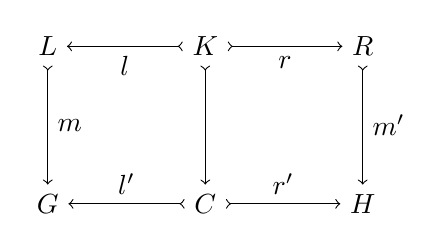
\begin{tikzpicture}
            % [node distance=15mm]
            \node (I) at (0,0) {$K$};
            \node (L)  at (-2,0) {$L$};
            \node (R)  at (2,0) {$R$};
            \node (G)  at (-2,-2) {$G$};
            \node (C)  at (0,-2) {$C$};
            \node (H)  at (2,-2) {$H$};
            \draw [>->] (I) to  node [midway,below] {$l$} (L);
            \draw [>->] (I) to  node [midway,below] {$r$} (R);
            \draw [>->] (L) to node [midway,right] {$m$} (G);
            \draw [>->] (I) to  node [midway,right] 
            % {$u$}
            {} (C);
            \draw [>->] (R) to  node [midway,right] 
            {$m'$}
            (H);
            \draw [>->] (C) to node [midway,above] {$l'$} (G);
            \draw [>->] (C) to node [midway,above] 
            {$r'$} 
            (H);
            % \node [at=($(I)!.5!(G)$)] {\normalfont PO};
            % \node [at=($(I)!.5!(H)$)] {\normalfont PO};
        \end{tikzpicture}
    }
\end{minipage}


\begin{flalign*}
    \operatorname{Mono}(X,G) &= 
    \operatorname{Mono}(X,G,l')
    \uplus
    \operatorname{Mono}(X,G,\lnot l',m) 
    \uplus
    \operatorname{Mono}(X,G,\lnot l',\lnot m)
    \\
    \operatorname{Mono}(X,H) &= 
    \operatorname{Mono}(X,H,r')
    \uplus
    \operatorname{Mono}(X,H,\lnot r',m') 
    \uplus
    \operatorname{Mono}(X,H,\lnot r',\lnot m')
\end{flalign*}
Thus, we have:
\begin{flalign*}
    \card{\operatorname{Mono}(X,G)} ={} &
    \card{\operatorname{Mono}(X,G,l')}
    +
    \card{\operatorname{Mono}(X,G,\lnot l',m)} \\
    &+
    \card{\operatorname{Mono}(X,G,\lnot l',\lnot m)}
    \\
    \card{\operatorname{Mono}(X,H)} ={} &
    \card{\operatorname{Mono}(X,H,r')} 
    +
    \card{\operatorname{Mono}(X,H,\lnot r',m')} \\
    &+\card{\operatorname{Mono}(X,H,\lnot r',\lnot m')}
\end{flalign*}
\noindent Using~\autoref{subgraph_counting:lem:decomp_w_u} 
(see \iflongversion
\textsection~\ref{subgraph_counting:proof:dcomp_w_u} 
\else
\cite[Lemma 27]{qiu2025termination}
\fi for a proof), we derive:
\begin{flalign*}
&\card{\operatorname{Mono}(X,G)} =
\card{\operatorname{Mono}(X,C)}
+
\card{\operatorname{Mono}(X,L, \lnot l)}
+
\card{\operatorname{Mono}(X,G, \lnot l',\lnot m)} 
 \\
 &\card{\operatorname{Mono}(X,H)} =
 \card{\operatorname{Mono}(X,C)}
 +
 \card{ \operatorname{Mono}(X,R, \lnot r) }
 +
 \card{ \operatorname{Mono}(X,H, \lnot r',\lnot m')}  
\end{flalign*}
\begin{lemma}
    \label{subgraph_counting:lem:decomp_w_u}
    \ \newline
    \noindent
    \begin{minipage}{0.69\textwidth}
        Let $X$ be a ruler-graph. For a pushout square as shown on the right, we have 
        % $\card{\operatorname{Mono}(X, B)} = \card{\operatorname{Mono}(X, D, \beta')}$ and $\card{\operatorname{Mono}(X, C, \lnot \beta)} = \card{\operatorname{Mono}(X, D, \lnot \beta', \alpha')}$.
        \begin{flalign*}
            \card{\operatorname{Mono}(X, B)} &= \card{\operatorname{Mono}(X, D, \beta')}
            \\
            \card{\operatorname{Mono}(X, C, \lnot \beta)} &= \card{\operatorname{Mono}(X, D, \lnot \beta', \alpha')}
        \end{flalign*}
    \end{minipage}
    \hfill
    \begin{minipage}{0.29\textwidth}
        \hfill
        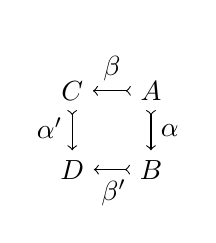
\begin{tikzpicture}
            \node (A) {$A$};
            \node [below of=A] (B) {$B$}; 
            \node [left of=A] (C) {$C$}; 
            \node [left of=B] (D) {$D$}; 
            \begin{scope}[nodes=rectangle]          
            \draw [>->] (A) to node [right,label,pos=0.5] {$\alpha$} (B);
            \draw [>->] (A) to node [above,label,pos=0.5] {$\beta$} (C);
            \draw [>->] (B) to node [below,label,pos=0.45] {$\beta'$} (D); 
            \draw [>->] (C) to node [left,label,pos=0.45] {$\alpha'$} (D);
            \end{scope}
        \end{tikzpicture}
    \end{minipage} 
\end{lemma}
Therefore, we obtain:
\begin{flalign*}
      &\card{\operatorname{Mono}(X,G)} -  \card{\operatorname{Mono}(X,H)} \\
     =& \card{\operatorname{Mono}(X,L, \lnot l)}- \card{\operatorname{Mono}(X,R, \lnot r)}  + \\ 
     &\card{\operatorname{Mono}(X,G, \lnot l',\lnot m)} - 
     \card{\operatorname{Mono}(X,H, \lnot r',\lnot m') } 
\end{flalign*}
By Lemma~\ref{subgraph_counting:lem:xlnlmxrnr} (see \iflongversion
    \textsection~\ref{subgraph_counting:proof:lem:xlnlmxrnr}
    \else
   ~\cite[Lemma 28]{qiu2025termination}
    \fi for a proof), it can be simplified to:
\begin{flalign*}
     &\card{\operatorname{Mono}(X,G)} -  \card{\operatorname{Mono}(X,H)} \\
    = & \card{\operatorname{Mono}(X,L)}- \card{\operatorname{Mono}(X,R)}  + \\ 
      & \card{\operatorname{Mono}(X,G, \lnot l',\lnot m)} - 
    \card{\operatorname{Mono}(X,H, \lnot r',\lnot m') } 
\end{flalign*}
\begin{lemma}
    \label{subgraph_counting:lem:xlnlmxrnr}
    Let $X$ be a graph. Let $L \overset{l}{\leftarrowtail} K \overset{r}{\rightarrowtail} R$ be an injective DPO graph rewriting rule. We have 
    \[
       \card{\operatorname{Mono}(X, L, \lnot l)}  - \card{\operatorname{Mono}(X, R, \lnot r)} 
       = 
       \card{\operatorname{Mono}(X, L)}  - \card{\operatorname{Mono}(X, R)} 
        \]
\end{lemma}
Consequently, the weight difference satisfies:
\begin{flalign*}
     &w_{s_\mathbb{X}}(G) - w_{s_\mathbb{X}}(H)\\
    \overset{\operatorname{def}}{=}&\sum_{X \in \mathbb{X}}^{}s_\mathbb{X}(X) * m_X(G) - \sum_{X \in \mathbb{X}}^{}s_\mathbb{X}(X) * m_X(H)\\
    \overset{\operatorname{def}}{=}&\sum_{X \in \mathbb{X}}^{}s_\mathbb{X}(X) * |\operatorname{Mono}(X,G)| - \sum_{X \in \mathbb{X}}^{}s_\mathbb{X}(X) * |\operatorname{Mono}(X,H)|\\
    =&\sum_{X \in \mathbb{X}}^{}s_\mathbb{X}(X) * \left( \card{\operatorname{Mono}(X,G)} -  \card{\operatorname{Mono}(X,H)} \right)\\
    =&\sum_{X \in \mathbb{X}}^{}s_\mathbb{X}(X) * \left(  \card{\operatorname{Mono}(X,L)}- \card{\operatorname{Mono}(X,R)} \right)+\\
       & \sum_{X \in \mathbb{X}}^{}s_\mathbb{X}(X) * \left( 
     \card{\operatorname{Mono}(X,G, \lnot l',\lnot m)} - 
    \card{\operatorname{Mono}(X,H, \lnot r',\lnot m') } \right)
\end{flalign*}
Since $\sum_{X \in \mathbb{X}}^{}s(X) * \left(  \card{\operatorname{Mono}(X,L)}- \card{\operatorname{Mono}(X,R)} \right)$ can be precisely computed, the key challenge is to establish a lower bound for
\begin{flalign*}
    % \label{ineq:key_challenge}
    \sum_{X \in \mathbb{X}}^{} s_\mathbb{X}(X) * 
         \left ( \card{\operatorname{Mono}(X,G, \lnot l',\lnot m)} - 
     \card{\operatorname{Mono}(X,H, \lnot r',\lnot m') } \right ) 
    % \label{ineq:ge0_sss}
\end{flalign*} 


\section{Non-increasing rules}
\label{subgraph_counting:sec:non-increasing}
% \noindent
% \begin{minipage}{0.7\textwidth}
%     % \setlength{\parindent}{1em}
%     Let \( \rho = (L \overset{l}{\leftarrowtail} K \overset{r}{\rightarrowtail} R) \) be an injective DPO rewriting rule. 
%     A DPO diagram as illustrated on the right defines a rewriting step using $\rho$ with injective match \( m \).
% \end{minipage}%
% \hfill 
% \begin{minipage}{0.3\textwidth}
%     \hfill
%     % \begin{figure}[htbp] 
%     %     \center
%         \begin{tikzpicture}
%             % [node distance=15mm]
%             \node (I) {$K$};
%             \node (L) [left of=I] {$L$};
%             \node (R) [right of=I] {$R$};
%             \node (G) [below of=L] {$G$};
%             \node (C) [below of=I] {$C$};
%             \node (H) [below of=R] {$H$};
%             \draw [>->] (I) to  node [midway,below] {$l$} (L);
%             \draw [>->] (I) to  node [midway,below] {$r$} (R);
%             \draw [>->] (L) to node [midway,right] {$m$} (G);
%             \draw [>->] (I) to  node [midway,right] 
%             % {$u$}
%             {} (C);
%             \draw [>->] (R) to  node [midway,right] 
%             % {$m'$}
%             {} (H);
%             \draw [>->] (C) to node [midway,above] {$l'$} (G);
%             \draw [>->] (C) to node [midway,above] 
%             % {$r'$} 
%             {}
%             (H);
%             % \node [at=($(I)!.5!(G)$)] {\normalfont PO};
%             % \node [at=($(I)!.5!(H)$)] {\normalfont PO};
%         \end{tikzpicture}
%             % \caption{}
%     %         \label{diag:set_dpo_intuition_1}
%     % \end{figure}
% \end{minipage}

% \noindent
% \begin{minipage}{0.5\textwidth}
%     % \setlength{\parindent}{1em}
%      It follows that the DPO diagram depicted on the right, where all morphisms are inclusion functions and $H'$ is a graph isomorphic to $H$, holds.
% \end{minipage}%
% \hfill 
% \begin{minipage}{0.5\textwidth}  
%     \hfill
%     \begin{tikzpicture}
%         [node distance=20mm]
%         \node (I) at (0,0) {$\operatorname{Im}(l \star m)$};
%         \node (L) at (-2,0) {$\operatorname{Im}(m)$};
%         \node (R) at (2,0) {$\operatorname{Im}(m')$};
%         \node (G) at (-2,-1) {$G$};
%         \node (C) at (0,-1) {$\operatorname{Im}(l')$};
%         \node (H) at (2,-1) {$H'$};
%         \draw [>->] (I) to  node [midway,above] {} (L);
%         \draw [>->] (I) to  node [midway,above] {} (R);
%         \draw [>->] (L) to node [midway,right] {} (G);
%         \draw [>->] (I) to  node [midway,right] {} (C);
%         \draw [>->] (R) to  node [midway,right] {} (H);
%         \draw [>->] (C) to node [midway,above] {} (G);
%         \draw [>->] (C) to node [midway,above] {} (H);
%         % \node [at=($(I)!.5!(G)$)] {\normalfont PO};
%         % \node [at=($(I)!.5!(H)$)] {\normalfont PO};
%       \end{tikzpicture}
% \end{minipage}


%  \noindent
%     \begin{minipage}{0.6\textwidth}
%         By viewing a graph as a set o f nodes and edges and graph monomorphisms as set injections, the above DPO diagram can be considered as a DPO diagram in the category of sets, illustrated on the right.
%     \end{minipage}
%     \hfill
%     \begin{minipage}{0.3\textwidth}
%           \hfill
%           \resizebox{\textwidth}{!}{
%             \begin{tikzpicture}
%               \coordinate (k) at (0, 0);
%               \draw[fill=white] ($(k)+(0,0)$) rectangle ($(k)+(0.5,0.5)$);
%               \node () at ($(k)+(0.25,0.25)$) {\( \mathrm{K} \)};
          
%               \coordinate (c) at (0, -2.2);
%               \draw[fill=blue!20]
%               ($(c)+(0,-0.5)$)
%               -- ($(c)+(0,0.5)$) 
%               -- ($(c)+(1,0.5)$) 
%               arc[start angle=0, end angle=-90, radius=1]
%               -- cycle;
%               \node () at ($(c)+(0.75,0.25)$) {\( \mathrm{C'} \)};
%               \draw[fill=white] ($(c)+(0,0)$) rectangle ($(c)+(0.5,0.5)$);
%               \node () at ($(c)+(0.25,0.25)$) {\( \mathrm{K} \)};
          
%               \coordinate (l) at (-3, 0);
%               \draw[fill=orange!20] ($(l)+(-0.5,0)$) rectangle ($(l)+(0.5,1)$);
%               \node () at ($(l)+(-0.23,0.25)$) {\( \mathrm{L'} \)};
%               \draw[fill=white] ($(l)+(0,0)$) rectangle ($(l)+(0.5,0.5)$);
%               \node () at ($(l)+(0.25,0.25)$) {\( \mathrm{K} \)};
          
%               \coordinate (g) at (-3, -2.2);
%               \draw[fill=blue!20]
%               ($(g)+(0,-0.5)$)
%               -- ($(g)+(0,0.5)$)
%               -- ($(g)+(1,0.5)$) 
%               arc[start angle=0, end angle=-90, radius=1]
%               -- cycle;
%               \draw[fill=orange!20] ($(g)+(-0.5,0)$) rectangle ($(g)+(0.5,1)$);
%               \node () at ($(g)+(0.75,0.25)$) {\( \mathrm{C'} \)};
%               \node () at ($(g)+(-0.23,0.25)$) {\( \mathrm{L'} \)};
%               \draw[fill=white] ($(g)+(0,0)$) rectangle ($(g)+(0.5,0.5)$);
%               \node () at ($(g)+(0.25,0.25)$) {\( \mathrm{K} \)};
          
%               \coordinate (r) at (3,0);
%               \draw[fill=red!20] ($(r)+(-0.5,0)$)
%                 -- ($(r)+(-0.5,0.5)$)
%                 -- ($(r)+(0,1)$)
%                 --  ($(r)+(0.5,1)$)
%                 -- ($(r)+(0.5,0)$)
%                 -- cycle;
%               \node () at ($(r)+(-0.23,0.25)$) {\( \mathrm{R'} \)};
%               \draw[fill=white] ($(r)+(0,0)$) rectangle ($(r)+(0.5,0.5)$);
%               \node () at ($(r)+(0.25,0.25)$) {\( \mathrm{K} \)};
          
%               \coordinate (h) at (3, -2.2);
%               \draw[fill=blue!20]
%               ($(h)+(0,-0.5)$)
%               -- ($(h)+(0,0.5)$)
%               -- ($(h)+(1,0.5)$) 
%               arc[start angle=0, end angle=-90, radius=1]
%               -- cycle;
%               \draw[fill=red!20] ($(h)+(-0.5,0)$)
%               -- ($(h)+(-0.5,0.5)$)
%               -- ($(h)+(0,1)$)
%               --  ($(h)+(0.5,1)$)
%               -- ($(h)+(0.5,0)$)
%               -- cycle;
%              \node () at ($(h)+(0.75,0.25)$) {\( \mathrm{C'} \)};
%              \draw[fill=white] ($(h)+(0,0)$) rectangle ($(h)+(0.5,0.5)$);
%              \node () at ($(h)+(0.25,0.25)$) {\( \mathrm{K} \)};
%              \node () at ($(h)+(-0.23,0.25)$) {\( \mathrm{R'} \)};
          
%               \node[ font=\huge] (kl) at ($(k)!0.5!(l)+(0.25,0.25)$)
%              %    {\( \overset{l}{\leftarrowtail} \)}
%                 {\( \leftarrowtail \)}
%                ; 
%               \node[ font=\huge] (kr) at ($(k)!0.5!(r)+(0.25,0.25)$)
%                {\( \rightarrowtail \)}
%                ;  
%               \node[ font=\huge] (cg) at ($(c)!0.5!(g)+(0.25,0.25)$) 
%               {\( \leftarrowtail \)}
%              ;  
%               \node[ font=\huge] (ch) at ($(c)!0.5!(h)+(0.25,0.25)$)
%                {\( \rightarrowtail \)}
%              ; 
%               \node[ font=\huge] (kc) at ($(k)!0.5!(c)+(0.2,0.4)$) {\( \downarrowtail \)}; 
%             %   \node[ font=\LARGE] () at ($(l)!0.5!(g)+(0.5,0.4)$) {$m$}; 
%               \node[ font=\huge] (lg) at ($(l)!0.5!(g)+(0.1,0.4)$) {\( \downarrowtail \)}; 
%               \node[ font=\huge] (rh) at ($(r)!0.5!(h)+(0.1,0.4)$) {\( \downarrowtail \)}; 
%             %   \node[ font=\LARGE] () at ($(r)!0.5!(h)+(0.55,0.4)$) {$m'$}; 
%             %   \node[ font=\LARGE] () at ($(k)!0.5!(c)+(0.5,0.4)$) {$u$}; 
%             \end{tikzpicture}
%         }
%     \end{minipage}
% \begin{minipage}{0.59\textwidth}
%     % \setlength{\parindent}{1em}
%     Let \( \rho = (L \overset{l}{\leftarrowtail} K \overset{r}{\rightarrowtail} R) \) be an injective DPO rewriting rule. 
%     A rewriting step using $\rho$ with injective match \( m \) is defined by a DPO diagram as shown on the upper right.
%      % \setlength{\parindent}{1em}
%      It follows that both squares in the diagram depicted on the middle right, where all morphisms are inclusion functions and $H'$ is a graph isomorphic to $H$, are pushouts.
%      By viewing a graph as a set of nodes and edges and graph monomorphisms as set injections, the DPO diagram on the middle right can be considered as a DPO diagram in the category of sets, illustrated on the lower right. In
% \end{minipage}%
% \hfill 
% \begin{minipage}{0.39\textwidth}
%     % \hfill 
%     %     \resizebox{0.7\textwidth}{!}{
%     %         \begin{tikzpicture}
%     %             % [node distance=15mm]
%     %             \node (I) {$K$};
%     %             \node (L) [left of=I] {$L$};
%     %             \node (R) [right of=I] {$R$};
%     %             \node (G) [below of=L] {$G$};
%     %             \node (C) [below of=I] {$C$};
%     %             \node (H) [below of=R] {$H$};
%     %             \draw [>->] (I) to  node [midway,below] {$l$} (L);
%     %             \draw [>->] (I) to  node [midway,below] {$r$} (R);
%     %             \draw [>->] (L) to node [midway,right] {$m$} (G);
%     %             \draw [>->] (I) to  node [midway,right] 
%     %             % {$u$}
%     %             {} (C);
%     %             \draw [>->] (R) to  node [midway,right] 
%     %             % {$m'$}
%     %             {} (H);
%     %             \draw [>->] (C) to node [midway,above] {$l'$} (G);
%     %             \draw [>->] (C) to node [midway,above] 
%     %             % {$r'$} 
%     %             {}
%     %             (H);
%     %             % \node [at=($(I)!.5!(G)$)] {\normalfont PO};
%     %             % \node [at=($(I)!.5!(H)$)] {\normalfont PO};
%     %         \end{tikzpicture}
%     %     }
%     \centering
%     \resizebox{0.7\textwidth}{!}{
%         \begin{tikzpicture}
%             % [node distance=15mm]
%             \node (I) at (0,0) {$K$};
%             \node (L)  at (-2,0) {$L$};
%             \node (R)  at (2,0) {$R$};
%             \node (G)  at (-2,-2) {$G$};
%             \node (C)  at (0,-2) {$C$};
%             \node (H)  at (2,-2) {$H$};
%             \draw [>->] (I) to  node [midway,below] {$l$} (L);
%             \draw [>->] (I) to  node [midway,below] {$r$} (R);
%             \draw [>->] (L) to node [midway,right] {$m$} (G);
%             \draw [>->] (I) to  node [midway,right] 
%             % {$u$}
%             {} (C);
%             \draw [>->] (R) to  node [midway,right] 
%             {$m'$}
%             (H);
%             \draw [>->] (C) to node [midway,above] {$l'$} (G);
%             \draw [>->] (C) to node [midway,above] 
%             % {$r'$} 
%             {}
%             (H);
%             % \node [at=($(I)!.5!(G)$)] {\normalfont PO};
%             % \node [at=($(I)!.5!(H)$)] {\normalfont PO};
%         \end{tikzpicture}
%     }

%         \resizebox{0.7\textwidth}{!}{
%             \begin{tikzpicture}
%                 [node distance=20mm]
%                 \node (I) at (0,0) {$\operatorname{Im}(l \star m)$};
%                 \node (L) at (-2,0) {$\operatorname{Im}(m)$};
%                 \node (R) at (2,0) {$\operatorname{Im}(m')$};
%                 \node (G) at (-2,-2) {$G$};
%                 \node (C) at (0,-2) {$\operatorname{Im}(l')$};
%                 \node (H) at (2,-2) {$H'$};
%                 \draw [>->] (I) to  node [midway,above] {} (L);
%                 \draw [>->] (I) to  node [midway,above] {} (R);
%                 \draw [>->] (L) to node [midway,right] {} (G);
%                 \draw [>->] (I) to  node [midway,right] {} (C);
%                 \draw [>->] (R) to  node [midway,right] {} (H);
%                 \draw [>->] (C) to node [midway,above] {} (G);
%                 \draw [>->] (C) to node [midway,above] {} (H);
%                 % \node [at=($(I)!.5!(G)$)] {\normalfont PO};
%                 % \node [at=($(I)!.5!(H)$)] {\normalfont PO};
%             \end{tikzpicture}
%         }

%           \resizebox{0.7\textwidth}{!}{
%             \begin{tikzpicture}
%                 \coordinate (k) at (0, 0);
%                 \draw[fill=white] ($(k)+(0,0)$) rectangle ($(k)+(0.5,0.5)$);
%                 \node () at ($(k)+(0.25,0.25)$) {\( \mathrm{K} \)};
            
%                 \coordinate (c) at (0, -2.2);
%                 \draw[fill=blue!20]
%                 ($(c)+(0,-0.5)$)
%                 -- ($(c)+(0,0.5)$) 
%                 -- ($(c)+(1,0.5)$) 
%                 arc[start angle=0, end angle=-90, radius=1]
%                 -- cycle;
%                 \node () at ($(c)+(0.75,0.25)$) {\( \mathrm{C'} \)};
%                 \draw[fill=white] ($(c)+(0,0)$) rectangle ($(c)+(0.5,0.5)$);
%                 \node () at ($(c)+(0.25,0.25)$) {\( \mathrm{K} \)};
            
%                 \coordinate (l) at (-3, 0);
%                 \draw[fill=orange!20] ($(l)+(-0.5,0)$) rectangle ($(l)+(0.5,1)$);
%                 \node () at ($(l)+(-0.23,0.25)$) {\( \mathrm{L'} \)};
%                 \draw[fill=white] ($(l)+(0,0)$) rectangle ($(l)+(0.5,0.5)$);
%                 \node () at ($(l)+(0.25,0.25)$) {\( \mathrm{K} \)};
            
%                 \coordinate (g) at (-3, -2.2);
%                 \draw[fill=blue!20]
%                 ($(g)+(0,-0.5)$)
%                 -- ($(g)+(0,0.5)$)
%                 -- ($(g)+(1,0.5)$) 
%                 arc[start angle=0, end angle=-90, radius=1]
%                 -- cycle;
%                 \draw[fill=orange!20] ($(g)+(-0.5,0)$) rectangle ($(g)+(0.5,1)$);
%                 \node () at ($(g)+(0.75,0.25)$) {\( \mathrm{C'} \)};
%                 \node () at ($(g)+(-0.23,0.25)$) {\( \mathrm{L'} \)};
%                 \draw[fill=white] ($(g)+(0,0)$) rectangle ($(g)+(0.5,0.5)$);
%                 \node () at ($(g)+(0.25,0.25)$) {\( \mathrm{K} \)};
            
%                 \coordinate (r) at (3,0);
%                 \draw[fill=red!20] ($(r)+(-0.5,0)$)
%                 -- ($(r)+(-0.5,0.5)$)
%                 -- ($(r)+(0,1)$)
%                 --  ($(r)+(0.5,1)$)
%                 -- ($(r)+(0.5,0)$)
%                 -- cycle;
%                 \node () at ($(r)+(-0.23,0.25)$) {\( \mathrm{R'} \)};
%                 \draw[fill=white] ($(r)+(0,0)$) rectangle ($(r)+(0.5,0.5)$);
%                 \node () at ($(r)+(0.25,0.25)$) {\( \mathrm{K} \)};
            
%                 \coordinate (h) at (3, -2.2);
%                 \draw[fill=blue!20]
%                 ($(h)+(0,-0.5)$)
%                 -- ($(h)+(0,0.5)$)
%                 -- ($(h)+(1,0.5)$) 
%                 arc[start angle=0, end angle=-90, radius=1]
%                 -- cycle;
%                 \draw[fill=red!20] ($(h)+(-0.5,0)$)
%                 -- ($(h)+(-0.5,0.5)$)
%                 -- ($(h)+(0,1)$)
%                 --  ($(h)+(0.5,1)$)
%                 -- ($(h)+(0.5,0)$)
%                 -- cycle;
%             \node () at ($(h)+(0.75,0.25)$) {\( \mathrm{C'} \)};
%             \draw[fill=white] ($(h)+(0,0)$) rectangle ($(h)+(0.5,0.5)$);
%             \node () at ($(h)+(0.25,0.25)$) {\( \mathrm{K} \)};
%             \node () at ($(h)+(-0.23,0.25)$) {\( \mathrm{R'} \)};
            
%                 \node[ font=\huge] (kl) at ($(k)!0.5!(l)+(0.25,0.25)$)
%             %    {\( \overset{l}{\leftarrowtail} \)}
%                 {\( \leftarrowtail \)}
%                 ; 
%                 \node[ font=\huge] (kr) at ($(k)!0.5!(r)+(0.25,0.25)$)
%                 {\( \rightarrowtail \)}
%                 ;  
%                 \node[ font=\huge] (cg) at ($(c)!0.5!(g)+(0.25,0.25)$) 
%                 {\( \leftarrowtail \)}
%             ;  
%                 \node[ font=\huge] (ch) at ($(c)!0.5!(h)+(0.25,0.25)$)
%                 {\( \rightarrowtail \)}
%             ; 
%                 \node[ font=\huge] (kc) at ($(k)!0.5!(c)+(0.2,0.4)$) {\( \downarrowtail \)}; 
%             %   \node[ font=\LARGE] () at ($(l)!0.5!(g)+(0.5,0.4)$) {$m$}; 
%                 \node[ font=\huge] (lg) at ($(l)!0.5!(g)+(0.1,0.4)$) {\( \downarrowtail \)}; 
%                 \node[ font=\huge] (rh) at ($(r)!0.5!(h)+(0.1,0.4)$) {\( \downarrowtail \)}; 
%             %   \node[ font=\LARGE] () at ($(r)!0.5!(h)+(0.55,0.4)$) {$m'$}; 
%             %   \node[ font=\LARGE] () at ($(k)!0.5!(c)+(0.5,0.4)$) {$u$}; 
%             \end{tikzpicture}
%           }
% \end{minipage}
% the lower right diagram, $L', C', R', K$ are mutually disjoint sets such that $K$, 
%          $K \uplus L'$, 
%          $K \uplus R'$, 
%          $K \uplus C'$, 
%          $L' \uplus K \uplus C'$ and 
%          $R' \uplus K \uplus C'$ 
%             are corresponding sets of 
%          $\operatorname{Im}(l \star m)$, 
%          $\operatorname{Im}(m)$, 
%          $\operatorname{Im}(m')$,
%          $\operatorname{Im}(l')$,
%          $G$ and
%          $H'$ respectively,
%          and all morphisms as inclusion functions.
%     % Up to isomorphism, we can further consider all morphisms as inclusion functions, illustrated on the right. In this visualization, $L',R',C',K$ are mutually disjoint sets with $L' \uplus K = L$, $R' \uplus K= R$, $C' \uplus K = C$, $G = L \cup C$ and $H = R \cup C$.
%     Thus, any subgraph of $G$ (resp. $H$) can be considered as a union of subgraphs of $C$ and $L$ (resp. $R$), up to isomorphism.
%     % \color{red}\begin{definition}
% %         Consider a rewriting step defined by the DPO diagram above. Let $X$ be a ruler-graph and $G$ a graph. An \textbf{$X$-occurrence} in $G$ is a subgraph of $G$ isomorphic to $X$. An \textbf{$X$-occurrence $x$ implicitly created by the rewriting step} is an \( X \)-occurrence in $H$ which is included neither in \( R \) nor in $C$. 
% %         Let $R' = x \cap R$, $C' = x \cap C$ and $h_{R'L}:R' \rightarrowtail L$ a monomorphism preserving interface elements. The \textbf{corresponding $X$-occurrence relative to $h_{R'L}$} of $x$ is the $X$-occurrence in $G$ defined by $h_{R'L}(R') \cup C'$.
% %         An \textbf{$X$-occurrence $x$ implicitly destroyed by the rewriting step} is an \( X \)-occurrence in $G$ which is included neither in \( L \) nor in $C$. 
% %     \end{definition}
% % \color{black}

% With the above DPO diagrams in mind, we define:

% \begin{definition}
%     \label{def:corresponding_occurrence}
%      An \textbf{$X$-occurrence} in $G$ is a subgraph of $G$ isomorphic to $X$. An \textbf{$X$-occurrence $x$ implicitly created by the rewriting step} is an \( X \)-occurrence in $H$ which is included neither in \( R \) nor in $C$. 
%       The occurrence $x$ can be decomposed as the union of graphs $x = R_x \cup C_x$ where $R_x = x \cap R$ and $C_x = x \cap C$. For every graph monomorphism $h : R_x \rightarrowtail L$ that preserves interface elements (i.e., \( h(k) = k \) for all \( k \in K \)), we define the \textbf{corresponding $X$-occurrence of $x$ relative to $h$} as the $X$-occurrence in $G$ given by $h(R_x) \cup C_x$.
%     An \textbf{$X$-occurrence implicitly destroyed by the rewriting step} is an \( X \)-occurrence in $G$ which is included neither in \( L \) nor in $C$.
% \end{definition}
We define the set \(D(R,X)\) of all subgraphs of \( R \) which, when glued along some common interface elements with a subgraph $C'$ of a context graph \( C \), can form an implicit \( X \)-occurrence.

\begin{definition}[Distinguished subgraphs of the right-hand side graph]
    \label{subgraph_counting:def:rx}
    Let \(X\) be a graph and 
    \(
        L \overset{l}{\leftarrowtail} K \overset{r}{\rightarrowtail} R
    \) an injective DPO rewriting rule.
    %  such that $l$ is edge-injective and $r$ is node-injective.
    The set \(D(R,X)\) consists of all subgraphs \( R' \subseteq R \)
    satisfying the following conditions:
    \newline
    \noindent
    \begin{minipage}{0.69\textwidth}\setlength{\parindent}{1em}
    \begin{itemize}
        \item a diagram as shown on the right where \(h_{K'K} \colon K' \rightarrowtail K \) and \(h_{R'R} \colon R' \rightarrowtail R \) are inclusion functions can be constructed,
        \item $R'$ is not a subgraph of $r(K)$,
        \item $R'$ is not isomorphic to $X$.
    \end{itemize}
    \end{minipage}
    \begin{minipage}{0.29\textwidth}
        \hfill
        \resizebox{0.9\textwidth}{!}{
        \begin{tikzpicture}[node distance=11mm]
            \node (k) {K};
            \node (r) [above=of k] {R};
            \node (r') [right=of r] {$R'$};
            \node (k') [right=of k] {K'};
            \node (x)  [right=of r'] {X};
            \node (c') [below=of x] {C'};
            \node () [at=($(r)!0.5!(k')$)] {PB};
            \node () [at=($(x)!0.5!(k')$)] {PO};
            \draw[>->] (k) -- (r) node[pos= .5, left] {$r$}; 
            \draw[>->] (r') -- (r) node[pos= .5, above] {$h_{R'R}$};
            \draw[>->] (k') -- (k) node[pos= .5, below] {$h_{K'K}$};
            \draw[>->] (k') -- (r');
            \draw[>->] (k') -- (c');
            \draw[>->] (c') -- (x);
            \draw[>->] (r') -- (x);
        \end{tikzpicture}
        }
    \end{minipage}
\end{definition}  
The first condition of the definition ensures that any $R' \in D(R,X)$ can be glued along some common interface elements with a subgraph $C'$ of a context graph \( C \) to form an \( X \)-occurrence. The second and third conditions ensure that such $X$-occurrences are included neither in \( C \) nor in \( R \), thereby guaranteeing that they are implicit.

% In another word, the set $D(R,X)$ contains all subgraphs $R''$ of $R$ which is not a subgraph of $K$ such that there exists a rewriting step defined by the diagram above such that $R'' \cup C''$ for a subgraph $C''$ of $C$ is an $X$-occurrence created by the rewriting step.

\begin{example}
    \label{subgraph_counting:ex:grsaa_rx}
    Consider the injective DPO rule from~\cite[Example 6]{bruggink2014termination}:  
    \begin{center} 
        \resizebox{0.7\textwidth}{!}{
        \begin{tikzpicture}
            \graphbox{$L$}{0mm}{0mm}{34mm}{15mm}{2mm}{-5mm}{
                \coordinate (o) at (0mm,-3mm); 
                \node[draw,circle] (l1) at ($(o)+(-10mm,0mm)$) {1};
                \node[draw,circle] (l2) at ($(l1)+(2,0)$) {2};
                \node[draw,circle] (l3) at ($(l1) + (1,0)$) {3};
                \draw[->] (l1) -- (l3) node[midway,above] {a};
                \draw[->] (l3) -- (l2) node[midway,above] {a};
            }     
            \graphbox{$K$}{40mm}{0mm}{24mm}{15mm}{2mm}{-5mm}{
                \coordinate (o) at (5mm,-3mm); 
                \node[draw,circle] (l1) at ($(o)+(-10mm,0mm)$) {1};
                \node[draw,circle] (l2) at ($(l1)+(1,0)$) {2};
                % \node[draw,circle] (l3) at ($(l1) + (1,0)$) {$\ $};
                % \draw[->] (l1) -- (l3) node[midway,above] {a};
                % \draw[->] (l3) -- (l2) node[midway,above] {a};
            }    
            \graphbox{$R$}{70mm}{0mm}{45mm}{15mm}{2mm}{-5mm}{
                \coordinate (o) at (-5mm,-3mm); 
                \node[draw,circle] (l1) at ($(o)+(-10mm,0mm)$) {1};
                \node[draw,circle] (l2) at ($(l1)+(3,0)$) {2};
                \node[draw,circle] (l3) at ($(l1) + (1,0)$) {4};
                \node[draw,circle] (l4) at ($(l1) + (2,0)$) {5};
                \draw[->] (l1) -- (l3) node[midway,above] {a};
                \draw[->] (l3) -- (l4) node[midway,above] {b};
                \draw[->] (l4) -- (l2) node[midway,above] {a};
            }    

            \node () at (37mm,-8mm) {$\leftarrowtail$};
            \node () at (67mm,-8mm) {$\rightarrowtail$};

            % \draw[>->] (51mm,2mm) -- (52mm,3mm);
        \end{tikzpicture}
        }
    \end{center}
    Let $X$ be \tikz[baseline=-0.5ex]{
        \node (x) at (0,0) {$\bullet$};
        \node (y) at (1,0) {$\bullet$ };
        \node (z) at (2,0) { $\bullet$};
        \draw[->] (x) -- (y) node[midway, above] {$a$};
        \draw[->] (y) -- (z) node[midway, above] {$a$};
    } and $R' \in D(R,X)$. 
    $R'$ is neither the empty graph nor isomorphic to $X$, by Conditions 2 and 3 of~\autoref{subgraph_counting:def:rx}. 
    Therefore, $R'$ must contain an interface node (either node 1 or node 2), because if it contains no interface node, Condition 1 of~\autoref{subgraph_counting:def:rx} would be violated due to $X$'s connectivity.
    Additionally, $R'$ must contain node 4 or node 5 to avoid being a subgraph of $r(K)$ (Condition 2). 
    Therefore, $R'$ must contain either $1 \overset{a}{\to} 4$ or $5 \overset{a}{\to} 2$, because if node 4 or node 5 is isolated, Condition 1 would be violated due to $X$'s connectivity.
    Furthermore, $R'$ must not contain $4 \overset{b}{\to} 5$ by Condition 1.
    The following graph is not in $D(R,X)$ because it violates Condition 1.
    \begin{center}
        \resizebox{0.24\textwidth}{!}{
            \begin{tikzpicture}
                \graphbox{}{70mm}{0mm}{45mm}{15mm}{2mm}{-5mm}{
                    \coordinate (o) at (-5mm,-3mm); 
                    \node[draw,circle] (l1) at ($(o)+(-10mm,0mm)$) {1};
                    \node[draw,circle] (l3) at ($(l1) + (1,0)$) {4};
                    \node[draw,circle] (l2) at ($(l1)+(3,0)$) {2};
                    \node[draw,circle] (l4) at ($(l1) + (2,0)$) {5};
                    \draw[->] (l4) -- (l2) node[midway,above] {a};
                    \draw[->] (l1) -- (l3) node[midway,above] {a};
                }    
            \end{tikzpicture}
        } 
    \end{center}
    Thus, $D(R,X)$ consists of the four graphs $R'_1$, $R'_2$, $R'_3$ and $R'_4$ shown below.
    For each graph, the construction of the pullback square in Condition 1 is demonstrated in~\autoref{example:grs_aa:has_more_left} and the construction of the pushout square required by Condition 1 is straightforward. 
    \begin{center}
        \resizebox{0.24\textwidth}{!}{
            \begin{tikzpicture}
                \graphbox{$R'_1$}{70mm}{0mm}{45mm}{15mm}{2mm}{-5mm}{
                    \coordinate (o) at (-5mm,-3mm); 
                    \node[circle] (l1) at ($(o)+(-10mm,0mm)$) {};
                    \node[draw,circle] (l2) at ($(l1)+(3,0)$) {2};
                    \node[draw,circle] (l4) at ($(l1) + (2,0)$) {5};
                    \draw[->] (l4) -- (l2) node[midway,above] {a};
                }    
            \end{tikzpicture}
        }
        \resizebox{0.24\textwidth}{!}{
            \begin{tikzpicture}
                \graphbox{$R'_2$}{70mm}{0mm}{45mm}{15mm}{2mm}{-5mm}{
                    \coordinate (o) at (-5mm,-3mm); 
                    \node[draw,circle] (l1) at ($(o)+(-10mm,0mm)$) {1};
                    \node[draw,circle] (l2) at ($(l1)+(3,0)$) {2};
                    \node[draw,circle] (l4) at ($(l1) + (2,0)$) {5};
                    \draw[->] (l4) -- (l2) node[midway,above] {a};
                }    
            \end{tikzpicture}
        } 
        \resizebox{0.24\textwidth}{!}{
            \begin{tikzpicture}
                \graphbox{$R'_3$}{70mm}{0mm}{45mm}{15mm}{2mm}{-5mm}{
                    \coordinate (o) at (-5mm,-3mm); 
                    \node[draw,circle] (l1) at ($(o)+(-10mm,0mm)$) {1};
                    \node[draw,circle] (l3) at ($(l1) + (1,0)$) {4};
                    \draw[->] (l1) -- (l3) node[midway,above] {a};
                }   
        \end{tikzpicture}
        } 
        \resizebox{0.24\textwidth}{!}{
            \begin{tikzpicture}
                \graphbox{$R'_4$}{70mm}{0mm}{45mm}{15mm}{2mm}{-5mm}{
                    \coordinate (o) at (-5mm,-3mm); 
                    \node[draw,circle] (l1) at ($(o)+(-10mm,0mm)$) {1};
                    \node[draw,circle] (l2) at ($(l1)+(3,0)$) {2};
                    \node[draw,circle] (l3) at ($(l1) + (1,0)$) {4};
                    \draw[->] (l1) -- (l3) node[midway,above] {a};
                }    
            \end{tikzpicture}
        }
    \end{center}
\end{example} 
 
\begin{example}
    \label{subgraph_counting:ex:rx_counter_ex}
    Let $X$ be the graph 
    \tikz[baseline=-0.5ex]{ 
            \node (x) at (0,0) {$\bullet$}; 
            \node (y) at (1,0) {$\bullet$};
            \node (z) at (2,0) {$\bullet$};
            \draw[->] (x) -- (y)   {};
            \draw[->] (y) -- (z)   {};
    }. Consider the following rule.
    \begin{center}
        \resizebox{0.6\textwidth}{!}{
            \begin{tikzpicture}
                \graphbox{$L$}{0mm}{0mm}{34mm}{15mm}{2mm}{-5mm}{
                    \coordinate (o) at (0mm,-3mm); 
                    \node[draw,circle] (l1) at ($(o)+(-10mm,0mm)$) {1};
                    % \node[draw,circle] (l2) at ($(l1)+(2,0)$) {2};
                    \node[draw,circle] (l3) at ($(l1) + (1,0)$) {2};
                    \draw[->] (l3) -- (l1) node[midway,above] {};
                    % \draw[->] (l3) -- (l2) node[midway,above] {a};
                }     
                \graphbox{$K$}{40mm}{0mm}{24mm}{15mm}{2mm}{-5mm}{
                    \coordinate (o) at (5mm,-3mm); 
                    \node[draw,circle] (l1) at ($(o)+(-10mm,0mm)$) {1};
                    \node[draw,circle] (l2) at ($(l1)+(1,0)$) {2};
                    % \node[draw,circle] (l3) at ($(l1) + (1,0)$) {$\ $};
                    \draw[->] (l2) -- (l1) node[midway,above] {};
                    % \draw[->] (l3) -- (l2) node[midway,above] {a};
                }    
                \graphbox{$R$}{70mm}{0mm}{40mm}{15mm}{2mm}{-5mm}{
                    \coordinate (o) at (-5mm,-3mm); 
                    \node[draw,circle] (l1) at ($(o)+(-10mm,0mm)$) {1};
                    % \node[draw,circle] (l2) at ($(l1)+(3,0)$) {2};
                    \node[draw,circle] (l3) at ($(l1) + (1,0)$) {2};
                    \node[draw,circle] (l4) at ($(l1) + (2,0)$) {3};
                    \draw[->] (l3) -- (l1) node[midway,above] {};
                    \draw[->] (l3) -- (l4) node[midway,above] {};
                    % \draw[->] (l4) -- (l2) node[midway,above] {a};
                }    
                \node () at (37mm,-8mm) {$\leftarrowtail$};
                \node () at (67mm,-8mm) {$\rightarrowtail$};
            \end{tikzpicture}
        }
    \end{center}
    Let $R' \in D(R,X)$. $R'$ must contain node 3, otherwise it would be a subgraph of $r(K)$, violating Condition 2 of~\autoref{subgraph_counting:def:rx}. Node 3 must be connected to an interface node, otherwise Condition 1 of~\autoref{subgraph_counting:def:rx} would be violated. Therefore, $R'$ must include \raisebox{2pt}{\scalebox{0.6}{\tikz[baseline=-0.5ex]{
        \node [draw,circle] (x) at (0,0) {2};
        \node[draw,circle] (y) at (1,0) {3};
        \draw[->] (x) -- (y) {};
    }}}.
    The graph $R$ is not in $D(R,X)$ because it violates Condition 1. Thus, the set \( D(R,X) \) consists of $R'_1$:
    \raisebox{2pt}{\scalebox{0.6}{\tikz[baseline=-0.5ex]{
        \node [draw,circle] (x) at (0,0) {2};
        \node[draw,circle] (y) at (1,0) {3};
        \draw[->] (x) -- (y) {};
    }}} and $R'_2$:
    \raisebox{2pt}{\scalebox{0.6}{\tikz[baseline=-0.5ex]{
        \node [draw,circle] (node1) at (-1,0) {1};
        \node [draw,circle] (x) at (0,0) {2};
        \node[draw,circle] (y) at (1,0) {3};
        \draw[->] (x) -- (y) {};
    }}}.
\end{example}
We define the notion of \( X \)-non-increasing rules. Intuitively, if a rule $\rho$ is $X$-non-increasing, then for any rewriting step using $\rho$, there exists an injective mapping from the set of \( X \)-occurrences implicitly created by the step to the set of \( X \)-occurrences implicitly destroyed by the step. This will be proved in~\autoref{subgraph_counting:lem:w_u_l_not_geq_r_not}.
\begin{definition}[Non-increasing rule]
    \label{subgraph_counting:def:creates_more_x_on_the_left}
    Let \(\rho = (L \overset{l}{\leftarrowtail} K \overset{r}{\rightarrowtail} R)\) be a rule and \(X\) a graph. 
    Let \( \Psi \) be a function associating $R' \in D(R,X)$ to a homomorphism in $\operatorname{Mono}(R',L)$.
    We say that \textbf{the number of occurrences of $X$ is non-increasing from left to right in any $\rho$-rewriting step under the mapping \(\Psi\)}
    (or that $\rho$ is $X$-\textbf{non-increasing} under $\Psi$. When $\Psi$ is clear from context or irrelevant to the discussion, we may simply say that $\rho$ is $X$-\textbf{non-increasing}.)
    % (or simply $\rho$ is $X$-non-increasing under \(\Psi\), or $\rho$ is $X$-non-increasing when \(\Psi\) is clear from the context or irrelevant to the discussion)
    if the following four conditions hold:
    \newline
    \vspace{1mm}
    \noindent
    \begin{minipage}{0.64\textwidth} 
    \begin{enumerate}
        \item For all $R' \in D(R,X)$, we can construct the diagram shown on the right, where all morphisms other than $\Psi(R')$, $l$ and $r$ are inclusion functions,
        % For all $R' \in D(R,X)$, in the diagram shown on the right, where $h_{R'R}$ is the inclusion function, both squares are pullbacks,
        % For all $R' \in D(R,X)$, there exists a morphism \(h_{R'L}: R' \rightarrowtail L \) such that \trackedtext{both squares in the diagram shown on the right are pullbacks}, where all morphisms other than $h_{R'L}$, $l$ and $r$ are inclusion functions,
        \item \label{def:non_increasing:non_clapse} For all $R' \in D(R,X)$, for all nodes and edges $x$ in $R'$, if $ x \notin \operatorname{Im}(r)$ then 
        $\Psi(R')(x) \notin \operatorname{Im}(l)$,
        % $h_{R'L}(r') \notin \operatorname{Im}(l)$,
        \item \label{def:non_increasing_rule_img_edges_distinct} For all $R',R'' \in D(R,X)$, for all edges $x$ in $R'$ and $y$ in $R''$, if $x \neq y$, then $\Psi(R')(x) \neq \Psi(R'')(y)$,
        \item If $X$ has isolated nodes, then for all $R',R'' \in D(R,X)$ and nodes $x$ and $y$ in $R'$ and $R''$ respectively, if $x \neq y$, then $\Psi(R')(x) \neq \Psi(R'')(y)$.
    \end{enumerate} 
    \end{minipage}
    \hfill
    \begin{minipage}{0.4\textwidth}
        % \hfill
        \begin{center}
            % \resizebox{0.9\textwidth}{!}{ 
                % \begin{tikzpicture}[rotate=90]
                %     \node (k) {K}; 
                %     \node (k') [above=of k] {$K'$};
                %     \node (l) [left=of k] {$L$};
                %     \node (rb) [above=of l] {$R'$};
                %     \node (r) [right=of k] {$R$};
                %     \node (rb') [above=of r] {$R'$};
                %     \draw[<-<]  (l) -- (k) node [midway,below] {l};
                %     \draw[<-<]  (r) -- (k) node [midway,below] {r};
                %     \draw[>->]  (k') -- (rb');
                %     \draw[>->]  (rb') -- (r);
                %     \draw[>->]  (k') -- (rb);
                %     \draw[>->]  (k') -- (k);
                %     \draw[>->]  (rb) -- (l) node [midway,above,sloped] {$h_{R'L}$};
                %     \node () [at=($(k)!0.5!(rb)$)] {PB};
                %     \node () [at=($(k)!0.5!(rb')$)] {PB};
                % \end{tikzpicture}
                \begin{tikzpicture} 
                    \node (k) {K}; 
                    \node (k') [left=of k] {$K'$};
                    \node (l) [above=of k] {$L$};
                    \node (rb) [left=of l] {$R'$};
                    \node (r) [below=of k] {$R$};
                    \node (rb') [left=of r] {$R'$};
                    \draw[<-<]  (l) -- (k) node [midway,right] {l};
                    \draw[<-<]  (r) -- (k) node [midway,right] {r};
                    \draw[>->]  (k') -- (rb');
                    \draw[>->]  (rb') -- (r);
                    \draw[>->]  (k') -- (rb);
                    \draw[>->]  (k') -- (k);
                    \draw[>->]  (rb) -- (l) node [midway,above] {$\Psi(R')$};
                    \node () [at=($(k)!0.5!(rb)$)] {PB};
                    \node () [at=($(k)!0.5!(rb')$)] {PB}; 
                \end{tikzpicture}
            % }
        \end{center}
    \end{minipage}
\end{definition}
% \begin{definition}[Non-increasing rule]
%     \label{def:creates_more_x_on_the_left}
%     Let \(\rho = (L \overset{l}{\leftarrowtail} K \overset{r}{\rightarrowtail} R)\) be a rule and \(X\) a ruler-graph. 
%     Rule \( \rho \) is \emph{\( X \)-non-increasing} if the following four conditions hold:
%     \newline
%     \vspace{1mm}
%     \noindent
%     \begin{minipage}{0.64\textwidth} 
%     \begin{enumerate}
%         \item For all $R' \in D(R,X)$, there exists a morphism \(h_{R'L}: R' \rightarrowtail L \) such that both squares in the diagram shown on the right are pullbacks, where all morphisms other than $h_{R'L}$, $l$ and $r$ are inclusion functions, 
%         \item \label{def:non_increasing:non_clapse} For all $R' \in D(R,X)$, for all node or edge $r'$ in $R'$, if $ r' \notin \operatorname{Im}(r)$ then $h_{R'L}(r') \notin \operatorname{Im}(l)$,
%         \item \label{def:non_increasing_rule_img_edges_distinct} For all $R',R'' \in D(R,X)$, for all edges $x \in R'$ and $y \in R''$, if $x \neq y$, then $h_{R'L}(x) \neq h_{R''L}(y)$,
%         \item If $X$ has isolated nodes, then for all $R',R'' \in D(R,X)$ and nodes $x \in R', y \in R''$, if $x \neq y$, then $h_{R'L}(x) \neq h_{R''L}(y)$.
%     \end{enumerate} 
%     \end{minipage}
%     \hfill
%     \begin{minipage}{0.4\textwidth}
%         % \hfill
%         \begin{center}
%             % \resizebox{0.9\textwidth}{!}{ 
%                 % \begin{tikzpicture}[rotate=90]
%                 %     \node (k) {K}; 
%                 %     \node (k') [above=of k] {$K'$};
%                 %     \node (l) [left=of k] {$L$};
%                 %     \node (rb) [above=of l] {$R'$};
%                 %     \node (r) [right=of k] {$R$};
%                 %     \node (rb') [above=of r] {$R'$};
%                 %     \draw[<-<]  (l) -- (k) node [midway,below] {l};
%                 %     \draw[<-<]  (r) -- (k) node [midway,below] {r};
%                 %     \draw[>->]  (k') -- (rb');
%                 %     \draw[>->]  (rb') -- (r);
%                 %     \draw[>->]  (k') -- (rb);
%                 %     \draw[>->]  (k') -- (k);
%                 %     \draw[>->]  (rb) -- (l) node [midway,above,sloped] {$h_{R'L}$};
%                 %     \node () [at=($(k)!0.5!(rb)$)] {PB};
%                 %     \node () [at=($(k)!0.5!(rb')$)] {PB};
%                 % \end{tikzpicture}
%                 \begin{tikzpicture} 
%                     \node (k) {K}; 
%                     \node (k') [left=of k] {$K'$};
%                     \node (l) [above=of k] {$L$};
%                     \node (rb) [left=of l] {$R'$};
%                     \node (r) [below=of k] {$R$};
%                     \node (rb') [left=of r] {$R'$};
%                     \draw[<-<]  (l) -- (k) node [midway,right] {l};
%                     \draw[<-<]  (r) -- (k) node [midway,right] {r};
%                     \draw[>->]  (k') -- (rb');
%                     \draw[>->]  (rb') -- (r);
%                     \draw[>->]  (k') -- (rb);
%                     \draw[>->]  (k') -- (k);
%                     \draw[>->]  (rb) -- (l) node [midway,above] {$h_{R'L}$};
%                     \node () [at=($(k)!0.5!(rb)$)] {PB};
%                     \node () [at=($(k)!0.5!(rb')$)] {PB};
%                 \end{tikzpicture}
%             % }
%         \end{center}
%     \end{minipage}

%     %  \begin{enumerate}
%     %     % \item[(2)] \label{def:non_increasing:non_clapse} For all node or arrow $r'$ in $R'$, if $ r' \notin \operatorname{Im}(r)$ then $h_{R'L}(r') \notin \operatorname{Im}(l)$,
%     %     % \item there exists a morphism $h_{R_XL}$ such that
%     %     %     \( h_{R'R_X} \star h_{R_XL} = h_{R'L} \) for all $R' \in D(R,X)$;
%     %     % \item[(3)] \label{def:non_increasing:edge_injective} For all $R',R'' \in D(R,X)$, for all edges $x \in R'$ and $y \in R''$, if $x \neq y$, then $h_{R'L}(x) \neq h_{R''L}(y)$,
%     %     %  \item $h$  is edge-injective 
%     %     % \item $\bigcup_{R' \in D(R,X)} h_{R'L}$ is an edge-injective morphism from $R_X$ to $L$;
%     %     % \item[(4)] \label{def:non_increasing:isolated_nodes} If $X$ has isolated nodes, then for all $R',R'' \in D(R,X)$ and nodes $x \in R', y \in R''$, if $x \neq y$, then $h_{R'L}(x) \neq h_{R''L}(y)$.
%     %     % \item $h$ is node-injective if $X$ has isolated nodes;
%     %  \end{enumerate}
%     %  \todo{est il util d'avoir "or arrow?" c'est une partie de edge injective, non ?}
% \end{definition} 
The first condition ensures that whenever $R' \in D(R,X)$ forms an $X$-occurrence in the result graph $H$, this occurrence has a corresponding $X$-occurrence relative to the morphism $h_{R'L}$ (as defined in~\autoref{def:x_occurrence}) in the host graph $G$.
The second condition guarantees that any $X$-occurrence implicitly created by the rewriting step has its corresponding $X$-occurrence not included in the context (Consequently, its corresponding $X$-occurrence is implicitly destroyed by the rewriting step). Counterexamples are provided in~\autoref{subgraph_counting:ex:cond_2_necessaire} and~\autoref{subgraph_counting:ex:cond_2_necessaire2}.
The third and fourth conditions ensure that distinct $X$-occurrences created implicitly have distinct corresponding $X$-occurrences.
Counterexamples for these conditions are given in~\autoref{subgraph_counting:ex:cond3_necessaire} and~\autoref{subgraph_counting:ex:cond4_necessaire}.

The following example shows an $X$-non-increasing rule. 
\begin{example}
    \label{example:grs_aa:has_more_left}
    Consider the rule presented
    in~\autoref{subgraph_counting:ex:grsaa_rx}. Let $X$ be \tikz[baseline=-0.5ex]{
        \node (x) at (0,0) {$\bullet$};
        \node (y) at (1,0) {$\bullet$};
        \node (z) at (2,0) {$\bullet$};
        \draw[->] (x) -- (y) node[midway, above] {$a$};
        \draw[<-] (z) -- (y) node[midway, above] {$a$};
    }.
    By~\autoref{subgraph_counting:ex:grsaa_rx}, the set \( D(R,X) \) consists of exactly four graphs: $R'_1$, $R'_2$, $R'_3$ and $R'_4$.
    The rule is $X$-non-increasing because the following diagrams can be constructed, and $h_{R'_1L}, h_{R'_2L}, h_{R'_3L}$ and $h_{R'_4L}$ satisfy all conditions in~\autoref{subgraph_counting:def:creates_more_x_on_the_left}. 
    %1
    \begin{center}
        \resizebox{0.7\textwidth}{!}{
            \begin{tikzpicture}
                \graphbox{$R'_1$}{0mm}{0mm}{34mm}{15mm}{2mm}{-5mm}{
                    \coordinate (o) at (0mm,-3mm); 
                    \node (l1) at ($(o)+(-10mm,0mm)$) {};
                    \node[draw,circle] (l2) at ($(l1)+(2,0)$) {2};
                    \node[draw,circle] (l3) at ($(l1) + (1,0)$) {5};
                    % \draw[->] (l1) -- (l3) node[midway,above] {a};
                    \draw[->] (l3) -- (l2) node[midway,above] {a};
                }     
                \graphbox{$K'$}{40mm}{0mm}{24mm}{15mm}{2mm}{-5mm}{
                    \coordinate (o) at (5mm,-3mm); 
                    \node (l1) at ($(o)+(-10mm,0mm)$) {};
                    \node[draw,circle] (l2) at ($(l1)+(1,0)$) {2};
                    % \node[draw,circle] (l3) at ($(l1) + (1,0)$) {$\ $};
                    % \draw[->] (l1) -- (l3) node[midway,above] {a};
                    % \draw[->] (l3) -- (l2) node[midway,above] {a};
                }    
                \graphbox{$R'_1$}{70mm}{0mm}{45mm}{15mm}{2mm}{-5mm}{
                    \coordinate (o) at (-5mm,-3mm); 
                    \node (l1) at ($(o)+(-10mm,0mm)$) {};
                    \node[draw,circle] (l2) at ($(l1)+(3,0)$) {2};
                    % \node[draw,circle] (l3) at ($(l1) + (1,0)$) {4};
                    \node[draw,circle] (l4) at ($(l1) + (2,0)$) {5};
                    % \draw[->] (l1) -- (l3) node[midway,above] {a};
                    % \draw[->] (l3) -- (l4) node[midway,above] {b};
                    \draw[->] (l4) -- (l2) node[midway,above] {a};
                }    
                \graphbox{$L$}{0mm}{-20mm}{34mm}{15mm}{2mm}{-5mm}{
                    \coordinate (o) at (0mm,-3mm); 
                    \node[draw,circle] (l1) at ($(o)+(-10mm,0mm)$) {1};
                    \node[draw,circle] (l2) at ($(l1)+(2,0)$) {2};
                    \node[draw,circle] (l3) at ($(l1) + (1,0)$) {5};
                    \draw[->] (l1) -- (l3) node[midway,above] {a};
                    \draw[->] (l3) -- (l2) node[midway,above] {a};
                }     
                \graphbox{$K$}{40mm}{-20mm}{24mm}{15mm}{2mm}{-5mm}{
                    \coordinate (o) at (5mm,-3mm); 
                    \node[draw,circle] (l1) at ($(o)+(-10mm,0mm)$) {1};
                    \node[draw,circle] (l2) at ($(l1)+(1,0)$) {2};
                    % \node[draw,circle] (l3) at ($(l1) + (1,0)$) {$\ $};
                    % \draw[->] (l1) -- (l3) node[midway,above] {a};
                    % \draw[->] (l3) -- (l2) node[midway,above] {a};
                }    
                \graphbox{$R$}{70mm}{-20mm}{45mm}{15mm}{2mm}{-5mm}{
                    \coordinate (o) at (-5mm,-3mm); 
                    \node[draw,circle] (l1) at ($(o)+(-10mm,0mm)$) {1};
                    \node[draw,circle] (l2) at ($(l1)+(3,0)$) {2};
                    \node[draw,circle] (l3) at ($(l1) + (1,0)$) {4};
                    \node[draw,circle] (l4) at ($(l1) + (2,0)$) {5};
                    \draw[->] (l1) -- (l3) node[midway,above] {a};
                    \draw[->] (l3) -- (l4) node[midway,above] {b};
                    \draw[->] (l4) -- (l2) node[midway,above] {a};
                }    
                \node () at (37mm,-8mm) {$\leftarrowtail$};
                \node () at (17mm,-17mm) {$\downarrowtail$};
                \node () at (52mm,-17mm) {$\downarrowtail$};
                \node () at (92mm,-17mm) {$\downarrowtail$};
                \node () at (37mm,-18mm) {\text{PB}};
                \node () at (68mm,-18mm) {\text{PB}};
                \node () at (67mm,-8mm) {$\rightarrowtail$};
                \node () at (37mm,-28mm) {$\leftarrowtail$};
                \node () at (67mm,-28mm) {$\rightarrowtail$};
            \end{tikzpicture}
        } 
    \end{center}   
    % 2
    \begin{center}
        \resizebox{0.7\textwidth}{!}{
            \begin{tikzpicture}
                \graphbox{$R'_2$}{0mm}{0mm}{34mm}{15mm}{2mm}{-5mm}{
                    \coordinate (o) at (0mm,-3mm); 
                    \node[draw,circle] (l1) at ($(o)+(-10mm,0mm)$) {1};
                    \node[draw,circle] (l2) at ($(l1)+(2,0)$) {2};
                    \node[draw,circle] (l3) at ($(l1) + (1,0)$) {5};
                    % \draw[->] (l1) -- (l3) node[midway,above] {a};
                    \draw[->] (l3) -- (l2) node[midway,above] {a};
                }     
                \graphbox{$K'$}{40mm}{0mm}{24mm}{15mm}{2mm}{-5mm}{
                    \coordinate (o) at (5mm,-3mm); 
                    \node[draw,circle] (l1) at ($(o)+(-10mm,0mm)$) {1};
                    \node[draw,circle] (l2) at ($(l1)+(1,0)$) {2};
                    % \node[draw,circle] (l3) at ($(l1) + (1,0)$) {$\ $};
                    % \draw[->] (l1) -- (l3) node[midway,above] {a};
                    % \draw[->] (l3) -- (l2) node[midway,above] {a};
                }    
                \graphbox{$R'_2$}{70mm}{0mm}{45mm}{15mm}{2mm}{-5mm}{
                    \coordinate (o) at (-5mm,-3mm); 
                    \node[draw,circle] (l1) at ($(o)+(-10mm,0mm)$) {1};
                    \node[draw,circle] (l2) at ($(l1)+(3,0)$) {2};
                    % \node[draw,circle] (l3) at ($(l1) + (1,0)$) {4};
                    \node[draw,circle] (l4) at ($(l1) + (2,0)$) {5};
                    % \draw[->] (l1) -- (l3) node[midway,above] {a};
                    % \draw[->] (l3) -- (l4) node[midway,above] {b};
                    \draw[->] (l4) -- (l2) node[midway,above] {a};
                }    
                \graphbox{$L$}{0mm}{-20mm}{34mm}{15mm}{2mm}{-5mm}{
                    \coordinate (o) at (0mm,-3mm); 
                    \node[draw,circle] (l1) at ($(o)+(-10mm,0mm)$) {1};
                    \node[draw,circle] (l2) at ($(l1)+(2,0)$) {2};
                    \node[draw,circle] (l3) at ($(l1) + (1,0)$) {5};
                    \draw[->] (l1) -- (l3) node[midway,above] {a};
                    \draw[->] (l3) -- (l2) node[midway,above] {a};
                }     
                \graphbox{$K$}{40mm}{-20mm}{24mm}{15mm}{2mm}{-5mm}{
                    \coordinate (o) at (5mm,-3mm); 
                    \node[draw,circle] (l1) at ($(o)+(-10mm,0mm)$) {1};
                    \node[draw,circle] (l2) at ($(l1)+(1,0)$) {2};
                    % \node[draw,circle] (l3) at ($(l1) + (1,0)$) {$\ $};
                    % \draw[->] (l1) -- (l3) node[midway,above] {a};
                    % \draw[->] (l3) -- (l2) node[midway,above] {a};
                }    
                \graphbox{$R$}{70mm}{-20mm}{45mm}{15mm}{2mm}{-5mm}{
                    \coordinate (o) at (-5mm,-3mm); 
                    \node[draw,circle] (l1) at ($(o)+(-10mm,0mm)$) {1};
                    \node[draw,circle] (l2) at ($(l1)+(3,0)$) {2};
                    \node[draw,circle] (l3) at ($(l1) + (1,0)$) {4};
                    \node[draw,circle] (l4) at ($(l1) + (2,0)$) {5};
                    \draw[->] (l1) -- (l3) node[midway,above] {a};
                    \draw[->] (l3) -- (l4) node[midway,above] {b};
                    \draw[->] (l4) -- (l2) node[midway,above] {a};
                }    
                \node () at (37mm,-8mm) {$\leftarrowtail$};
                \node () at (17mm,-17mm) {$\downarrowtail$};
                \node () at (52mm,-17mm) {$\downarrowtail$};
                \node () at (92mm,-17mm) {$\downarrowtail$};
                \node () at (37mm,-18mm) {\text{PB}};
                \node () at (68mm,-18mm) {\text{PB}};
                \node () at (67mm,-8mm) {$\rightarrowtail$};
                \node () at (37mm,-28mm) {$\leftarrowtail$};
                \node () at (67mm,-28mm) {$\rightarrowtail$};
            \end{tikzpicture}
        } 
    \end{center}
    %3
    \begin{center}
        \resizebox{0.7\textwidth}{!}{
            \begin{tikzpicture}
                \graphbox{$R'_3$}{0mm}{0mm}{34mm}{15mm}{2mm}{-5mm}{
                    \coordinate (o) at (0mm,-3mm); 
                    \node[draw,circle] (l1) at ($(o)+(-10mm,0mm)$) {1};
                    % \node[draw,circle] (l2) at ($(l1)+(2,0)$) {2};
                    \node[draw,circle] (l3) at ($(l1) + (1,0)$) {4};
                    \draw[->] (l1) -- (l3) node[midway,above] {a};
                    % \draw[->] (l3) -- (l2) node[midway,above] {a};
                }     
                \graphbox{$K'$}{40mm}{0mm}{24mm}{15mm}{2mm}{-5mm}{
                    \coordinate (o) at (5mm,-3mm); 
                    \node[draw,circle] (l1) at ($(o)+(-10mm,0mm)$) {1};
                    % \node[draw,circle] (l2) at ($(l1)+(1,0)$) {2};
                    % \node[draw,circle] (l3) at ($(l1) + (1,0)$) {$\ $};
                    % \draw[->] (l1) -- (l3) node[midway,above] {a};
                    % \draw[->] (l3) -- (l2) node[midway,above] {a};
                }     
                \graphbox{$R'_3$}{70mm}{0mm}{45mm}{15mm}{2mm}{-5mm}{
                    \coordinate (o) at (-5mm,-3mm); 
                    \node[draw,circle] (l1) at ($(o)+(-10mm,0mm)$) {1};
                    % \node[draw,circle] (l2) at ($(l1)+(3,0)$) {4};
                    \node[draw,circle] (l3) at ($(l1) + (1,0)$) {4};
                    % \node[draw,circle] (l4) at ($(l1) + (2,0)$) {5};
                    \draw[->] (l1) -- (l3) node[midway,above] {a};
                    % \draw[->] (l3) -- (l4) node[midway,above] {b};
                    % \draw[->] (l4) -- (l2) node[midway,above] {a};
                }    
                \graphbox{$L$}{0mm}{-20mm}{34mm}{15mm}{2mm}{-5mm}{
                    \coordinate (o) at (0mm,-3mm); 
                    \node[draw,circle] (l1) at ($(o)+(-10mm,0mm)$) {1};
                    \node[draw,circle] (l2) at ($(l1)+(2,0)$) {2};
                    \node[draw,circle] (l3) at ($(l1) + (1,0)$) {4};
                    \draw[->] (l1) -- (l3) node[midway,above] {a};
                    \draw[->] (l3) -- (l2) node[midway,above] {a};
                }     
                \graphbox{$K$}{40mm}{-20mm}{24mm}{15mm}{2mm}{-5mm}{
                    \coordinate (o) at (5mm,-3mm); 
                    \node[draw,circle] (l1) at ($(o)+(-10mm,0mm)$) {1};
                    \node[draw,circle] (l2) at ($(l1)+(1,0)$) {2};
                    % \node[draw,circle] (l3) at ($(l1) + (1,0)$) {$\ $};
                    % \draw[->] (l1) -- (l3) node[midway,above] {a};
                    % \draw[->] (l3) -- (l2) node[midway,above] {a};
                }    
                \graphbox{$R$}{70mm}{-20mm}{45mm}{15mm}{2mm}{-5mm}{
                    \coordinate (o) at (-5mm,-3mm); 
                    \node[draw,circle] (l1) at ($(o)+(-10mm,0mm)$) {1};
                    \node[draw,circle] (l2) at ($(l1)+(3,0)$) {2};
                    \node[draw,circle] (l3) at ($(l1) + (1,0)$) {4};
                    \node[draw,circle] (l4) at ($(l1) + (2,0)$) {5};
                    \draw[->] (l1) -- (l3) node[midway,above] {a};
                    \draw[->] (l3) -- (l4) node[midway,above] {b};
                    \draw[->] (l4) -- (l2) node[midway,above] {a};
                }    
                \node () at (37mm,-8mm) {$\leftarrowtail$};
                \node () at (17mm,-17mm) {$\downarrowtail$};
                \node () at (52mm,-17mm) {$\downarrowtail$};
                \node () at (92mm,-17mm) {$\downarrowtail$};
                \node () at (37mm,-18mm) {\text{PB}};
                \node () at (68mm,-18mm) {\text{PB}};
                \node () at (67mm,-8mm) {$\rightarrowtail$};
                \node () at (37mm,-28mm) {$\leftarrowtail$};
                \node () at (67mm,-28mm) {$\rightarrowtail$};
            \end{tikzpicture}
        } 
    \end{center}
    %4
    \begin{center}
        \resizebox{0.7\textwidth}{!}{
            \begin{tikzpicture}
                \graphbox{$R'_4$}{0mm}{0mm}{34mm}{15mm}{2mm}{-5mm}{
                    \coordinate (o) at (0mm,-3mm); 
                    \node[draw,circle] (l1) at ($(o)+(-10mm,0mm)$) {1};
                    \node[draw,circle] (l2) at ($(l1)+(2,0)$) {2};
                    \node[draw,circle] (l3) at ($(l1) + (1,0)$) {4};
                    \draw[->] (l1) -- (l3) node[midway,above] {a};
                    % \draw[->] (l3) -- (l2) node[midway,above] {a};
                }     
                \graphbox{$K'$}{40mm}{0mm}{24mm}{15mm}{2mm}{-5mm}{
                    \coordinate (o) at (5mm,-3mm); 
                    \node[draw,circle] (l1) at ($(o)+(-10mm,0mm)$) {1};
                    \node[draw,circle] (l2) at ($(l1)+(1,0)$) {2};
                    % \node[draw,circle] (l3) at ($(l1) + (1,0)$) {$\ $};
                    % \draw[->] (l1) -- (l3) node[midway,above] {a};
                    % \draw[->] (l3) -- (l2) node[midway,above] {a};
                }     
                \graphbox{$R'_4$}{70mm}{0mm}{45mm}{15mm}{2mm}{-5mm}{
                    \coordinate (o) at (-5mm,-3mm); 
                    \node[draw,circle] (l1) at ($(o)+(-10mm,0mm)$) {1};
                    \node[draw,circle] (l2) at ($(l1)+(3,0)$) {2};
                    \node[draw,circle] (l3) at ($(l1) + (1,0)$) {4};
                    % \node[draw,circle] (l4) at ($(l1) + (2,0)$) {5};
                    \draw[->] (l1) -- (l3) node[midway,above] {a};
                    % \draw[->] (l3) -- (l4) node[midway,above] {b};
                    % \draw[->] (l4) -- (l2) node[midway,above] {a};
                }    
                \graphbox{$L$}{0mm}{-20mm}{34mm}{15mm}{2mm}{-5mm}{
                    \coordinate (o) at (0mm,-3mm); 
                    \node[draw,circle] (l1) at ($(o)+(-10mm,0mm)$) {1};
                    \node[draw,circle] (l2) at ($(l1)+(2,0)$) {2};
                    \node[draw,circle] (l3) at ($(l1) + (1,0)$) {4};
                    \draw[->] (l1) -- (l3) node[midway,above] {a};
                    \draw[->] (l3) -- (l2) node[midway,above] {a};
                }     
                \graphbox{$K$}{40mm}{-20mm}{24mm}{15mm}{2mm}{-5mm}{
                    \coordinate (o) at (5mm,-3mm); 
                    \node[draw,circle] (l1) at ($(o)+(-10mm,0mm)$) {1};
                    \node[draw,circle] (l2) at ($(l1)+(1,0)$) {2};
                    % \node[draw,circle] (l3) at ($(l1) + (1,0)$) {$\ $};
                    % \draw[->] (l1) -- (l3) node[midway,above] {a};
                    % \draw[->] (l3) -- (l2) node[midway,above] {a};
                }    
                \graphbox{$R$}{70mm}{-20mm}{45mm}{15mm}{2mm}{-5mm}{
                    \coordinate (o) at (-5mm,-3mm); 
                    \node[draw,circle] (l1) at ($(o)+(-10mm,0mm)$) {1};
                    \node[draw,circle] (l2) at ($(l1)+(3,0)$) {2};
                    \node[draw,circle] (l3) at ($(l1) + (1,0)$) {4};
                    \node[draw,circle] (l4) at ($(l1) + (2,0)$) {5};
                    \draw[->] (l1) -- (l3) node[midway,above] {a};
                    \draw[->] (l3) -- (l4) node[midway,above] {b};
                    \draw[->] (l4) -- (l2) node[midway,above] {a};
                }    
                \node () at (37mm,-8mm) {$\leftarrowtail$};
                \node () at (17mm,-17mm) {$\downarrowtail$};
                \node () at (52mm,-17mm) {$\downarrowtail$};
                \node () at (92mm,-17mm) {$\downarrowtail$};
                \node () at (37mm,-18mm) {\text{PB}};
                \node () at (68mm,-18mm) {\text{PB}};
                \node () at (67mm,-8mm) {$\rightarrowtail$};
                \node () at (37mm,-28mm) {$\leftarrowtail$};
                \node () at (67mm,-28mm) {$\rightarrowtail$};
            \end{tikzpicture}
        } 
    \end{center}
    % with the following morphisms $h_{R'L}$ and $h_{R''L}$:
    % \begin{center}
    %     \resizebox{0.6\textwidth}{!}{
    %         \begin{tikzpicture}
    %             \graphbox{$R'$}{0}{0}{44mm}{15mm}{2mm}{-5mm}{
    %                 \coordinate (o) at (-5mm,-3mm); 
    %                 \node[draw,circle] (l1) at ($(o)+(-10mm,0mm)$) {1};
    %                 \node[draw,circle] (l3) at ($(l1) + (1,0)$) {4};
    %                 \draw[->] (l1) -- (l3) node[midway,above] {a};
    %             } 
    %             \graphbox{$L$}{60mm}{0mm}{34mm}{15mm}{2mm}{-5mm}{
    %                 \coordinate (o) at (0mm,-3mm); 
    %                 \node[draw,circle] (l1) at ($(o)+(-10mm,0mm)$) {1};
    %                 \node[draw,circle] (l2) at ($(l1)+(2,0)$) {};
    %                 \node[draw,circle] (l3) at ($(l1) + (1,0)$) {4};
    %                 \draw[->] (l1) -- (l3) node[midway,above] {a};
    %                 \draw[->] (l3) -- (l2) node[midway,above] {a};
    %             }    
    %         \node () at (52mm,-8mm) {$\rightarrowtail$};
    %         \end{tikzpicture}
    %      }
    %     \end{center}
    %     \begin{center}
    %         \resizebox{0.6\textwidth}{!}{
    %             \begin{tikzpicture}
    %                 \graphbox{$R''$}{0}{0}{44mm}{15mm}{2mm}{-5mm}{
    %                     \coordinate (o) at (-5mm,-3mm); 
    %                     \node[] (l1) at ($(o)+(-10mm,0mm)$) {};
    %                     \node[draw,circle] (l2) at ($(l1)+(3,0)$) {2};
    %                     \node[draw,circle] (l4) at ($(l1) + (2,0)$) {5};
    %                     \draw[->] (l4) -- (l2) node[midway,above] {a};
    %                 } 
    %                 \graphbox{$L$}{60mm}{0mm}{34mm}{15mm}{2mm}{-5mm}{
    %                     \coordinate (o) at (0mm,-3mm); 
    %                     \node[draw,circle] (l1) at ($(o)+(-10mm,0mm)$) {};
    %                     \node[draw,circle] (l2) at ($(l1)+(2,0)$) {2};
    %                     \node[draw,circle] (l3) at ($(l1) + (1,0)$) {5};
    %                     \draw[->] (l1) -- (l3) node[midway,above] {a};
    %                     \draw[->] (l3) -- (l2) node[midway,above] {a};
    %                 }    
    %             \node () at (52mm,-8mm) {$\rightarrowtail$};
    %             \end{tikzpicture}
    %         }
    %     \end{center}
    % To illustrate the property captured by~\autoref{def:creates_more_x_on_the_left},
    % consider the rewriting step defined by the DPO diagram below. Whenever an element $R' \in D(R,X)$ forms an \( X \)-occurrence in $H$ that is included neither in \( R \) nor $C$ with $C' \subseteq C$, the graph
    % \( \operatorname{\Psi(R')} \subseteq L\) forms an \( X \)-occurrence in $G$ with $C'$ that is included neither in \( L \) nor $C$.
    % Furthermore, distinct $X$-occurrences in $H$ that are included neither in \( R \) nor $C$ have distinct corresponding $X$-occurrences in $G$ that are included neither in \( L \) nor $C$.
    To illustrate the $X$-non-increasing property captured by~\autoref{subgraph_counting:def:creates_more_x_on_the_left},
    consider the rewriting step defined by the DPO diagram below. Whenever \( R'_i \) (for \( 1 \leq i \leq 4 \)) forms an \( X \)-occurrence $x$ in $H$ that is included neither in \( R \) nor $C$ with a subgraph $C' \subseteq C \cap x \subseteq C$, the graph
    \( \operatorname{\Psi(R')} \subseteq L\) forms a \( X \)-occurrence in $G$ with $C'$ that is included neither in \( L \) nor $C$.
    Furthermore, distinct $X$-occurrences in $H$ that are included neither in \( R \) nor $C$ have distinct corresponding $X$-occurrences in $G$ that are included neither in \( L \) nor $C$.
    \begin{center} 
        \resizebox{0.7\textwidth}{!}{
        \begin{tikzpicture}
            \graphbox{\( L \)}{0mm}{5mm}{34mm}{20mm}{2mm}{-5mm}{
                \coordinate (o) at (0mm,-8mm); 
                \node[draw,circle] (l1) at ($(o)+(-10mm,0mm)$) {1};
                \node[draw,circle] (l2) at ($(l1)+(2,0)$) {2};
                \node[draw,circle] (l3) at ($(l1) + (1,0)$) {3};
                \draw[] (l1) -- (l3) node[midway,above] {a};
                \draw[] (l3) -- (l2) node[midway,above] {a};
            } 

            \graphbox{\( K \)}{40mm}{5mm}{34mm}{20mm}{2mm}{-5mm}{
                \coordinate (o) at (0mm,-8mm); 
                \node[draw,circle] (l1) at ($(o)+(-10mm,0mm)$) {1};
                \node[draw,circle] (l2) at ($(l1)+(2,0)$) {2};
            }  

            \graphbox{\( R \)}{80mm}{5mm}{45mm}{20mm}{2mm}{-5mm}{
                \coordinate (o) at (-5mm,-8mm); 
                \node[draw,circle] (l1) at ($(o)+(-10mm,0mm)$) {1};
                \node[draw,circle] (l2) at ($(l1)+(3,0)$) {2};
                \node[draw,circle] (l3) at ($(l1) + (1,0)$) {4};
                \node[draw,circle] (l4) at ($(l1) + (2,0)$) {5};
                \draw[ ] (l1) -- (l3) node[midway,above] {a};
                \draw[ ] (l3) -- (l4) node[midway,above] {b};
                \draw[ ] (l4) -- (l2) node[midway,above] {a};
            }    

            \graphbox{\( G \)}{0mm}{-22mm}{34mm}{30mm}{2mm}{-10mm}{
                \coordinate (o) at (0mm,-3mm); 
                \node[draw,circle] (l1) at ($(o)+(-10mm,0mm)$) {1};
                \node[draw,circle] (l2) at ($(l1)+(2,0)$) {2};
                \node[draw,circle] (l3) at ($(l1) + (1,0)$) {3};
                \node[draw,circle] (l4) at ($(l2) + (0,-1)$) {6};
                \draw[] (l1) -- (l3) node[midway,above] {a};
                \draw[] (l3) -- (l2) node[midway,above] {a};
                \draw[ ] (l2) -- (l4) node[midway,right] {a};
                \node[draw,circle] (l6) at ($(l1) + (0,-1)$) {7};
                \draw[] (l1) -- (l6) node[midway,left] {a};
            }    

            \graphbox{\( C  \)}{40mm}{-22mm}{34mm}{30mm}{2mm}{-10mm}{
                \coordinate (o) at (0mm,-3mm); 
                \node[draw,circle] (l1) at ($(o)+(-10mm,0mm)$) {1};
                \node[draw,circle] (l2) at ($(l1)+(2,0)$) {2};
                \node[draw,circle] (l4) at ($(l2) + (0,-1)$) {6};
                \draw[ ] (l2) -- (l4) node[midway,right] {a};
                \node[ draw,circle] (l6) at ($(l1) + (0,-1)$) {7};
                \draw[ ] (l1) -- (l6) node[midway,left] {a};
            }    

            \graphbox{\( H  \)}{80mm}{-22mm}{45mm}{30mm}{2mm}{-10mm}{
                \coordinate (o) at (-5mm,-3mm); 
                \node[draw,circle] (l1) at ($(o)+(-10mm,0mm)$) {1};
                \node[draw,circle] (l2) at ($(l1)+(3,0)$) {2};
                \node[draw,circle] (l3) at ($(l1) + (1,0)$) {4};
                \node[draw,circle] (l4) at ($(l1) + (2,0)$) {5};
                \node[ draw,circle] (l5) at ($(l2) + (0,-1)$) {6};
                \node[ draw,circle] (l6) at ($(l1) + (0,-1)$) {7};
                \draw[ ] (l1) -- (l6) node[midway,left] {a};
                \draw[] (l1) -- (l3) node[midway,above] {a};
                \draw[] (l3) -- (l4) node[midway,above] {b};
                \draw[ ] (l4) -- (l2) node[midway,above] {a};
                \draw[ ] (l2) -- (l5) node[midway,right] {a};
            }    
            \node () at (37mm,-18mm) {\text{PO}};
            \node () at (78mm,-18mm) {\text{PO}};
            \node () at (37mm,-8mm) {\( \leftarrowtail \)}; % K -> L
            \node () at (77mm,-8mm) {\( \rightarrowtail \)}; % K -> R
            \node () at (17mm,-18mm) {\( m\ \downarrowtail \)};
            \node () at (37mm,-33mm) {\( \leftarrowtail \)};
            \node () at (52mm,-18mm) {\( \downarrowtail \)};
            \node () at (92mm,-18mm) {\( \downarrowtail \)};
            \node () at (77mm,-33mm) {\( \rightarrowtail \)}; % C -> H
        \end{tikzpicture}
        }
    \end{center}
\end{example}

% cond 2 necessaire  1
\begin{example} 
    \label{subgraph_counting:ex:cond_2_necessaire}
    Let $X$ be the graph 
    \tikz[baseline=-0.5ex]{ 
            \node (x) at (0,0) {$\bullet$}; 
            \node (y) at (1,0) {$\bullet$};
            \node (z) at (2,0) {$\bullet$};
            \draw[->] (x) -- (y)   {};
            \draw[->] (y) -- (z)   {};
    }. The following rewriting rule is potentially $X$-increasing.
    \begin{center}
        \resizebox{0.7\textwidth}{!}{
            \begin{tikzpicture}
                \graphbox{$L$}{0mm}{0mm}{34mm}{15mm}{2mm}{-5mm}{
                    \coordinate (o) at (0mm,-3mm); 
                    \node[draw,circle] (l1) at ($(o)+(-10mm,0mm)$) {1};
                    % \node[draw,circle] (l2) at ($(l1)+(2,0)$) {2};
                    \node[draw,circle] (l3) at ($(l1) + (1,0)$) {2};
                    \draw[->] (l3) -- (l1) node[midway,above] {};
                    % \draw[->] (l3) -- (l2) node[midway,above] {a};
                }     
                \graphbox{$K$}{40mm}{0mm}{24mm}{15mm}{2mm}{-5mm}{
                    \coordinate (o) at (5mm,-3mm); 
                    \node[draw,circle] (l1) at ($(o)+(-10mm,0mm)$) {1};
                    \node[draw,circle] (l2) at ($(l1)+(1,0)$) {2};
                    % \node[draw,circle] (l3) at ($(l1) + (1,0)$) {$\ $};
                    \draw[->] (l2) -- (l1) node[midway,above] {};
                    % \draw[->] (l3) -- (l2) node[midway,above] {a};
                }    
                \graphbox{$R$}{70mm}{0mm}{45mm}{15mm}{2mm}{-5mm}{
                    \coordinate (o) at (-5mm,-3mm); 
                    \node[draw,circle] (l1) at ($(o)+(-10mm,0mm)$) {1};
                    % \node[draw,circle] (l2) at ($(l1)+(3,0)$) {2};
                    \node[draw,circle] (l3) at ($(l1) + (1,0)$) {2};
                    \node[draw,circle] (l4) at ($(l1) + (2,0)$) {3};
                    \draw[->] (l3) -- (l1) node[midway,above] {};
                    \draw[->] (l3) -- (l4) node[midway,above] {};
                    % \draw[->] (l4) -- (l2) node[midway,above] {a};
                }    
                \node () at (37mm,-8mm) {$\leftarrowtail$};
                \node () at (67mm,-8mm) {$\rightarrowtail$};
            \end{tikzpicture}
        }
    \end{center}
    As shown in~\autoref{subgraph_counting:ex:rx_counter_ex}, \( D(R,X) \) contains the graph $R'$:
    \raisebox{2pt}{
        \scalebox{0.6}{\tikz[baseline=-0.5ex]{
        \node [draw,circle] (x) at (0,0) {2};
        \node[draw,circle] (y) at (1,0) {3};
        \draw[->] (x) -- (y) {};
    }}}. The unique monomorphism $h_{R'L}:R' \rightarrowtail L$ fails the second condition of~\autoref{subgraph_counting:def:creates_more_x_on_the_left}. 
    %  as illustrated below 
    % \begin{center}
    %     \resizebox{0.6\textwidth}{!}{
    %     \begin{tikzpicture}
    %             \graphbox{$R'$}{40mm}{-20mm}{24mm}{15mm}{2mm}{-5mm}{
    %                 \coordinate (o) at (5mm,-3mm); 
    %                 \node[draw,circle] (l1) at ($(o)+(-10mm,0mm)$) {2};
    %                 \node[draw,circle] (l2) at ($(l1)+(1,0)$) {3};
    %                 % \node[draw,circle] (l3) at ($(l1) + (1,0)$) {$\ $};
    %                 \draw[->] (l1) -- (l2) node[midway,above] {};
    %                 % \draw[->] (l3) -- (l2) node[midway,above] {a};
    %             }    
    %             \graphbox{$L$}{70mm}{-20mm}{45mm}{15mm}{2mm}{-5mm}{
    %                 \coordinate (o) at (-5mm,-3mm); 
    %                 \node[draw,circle] (l1) at ($(o)+(-10mm,0mm)$) {3};
    %                 % \node[draw,circle] (l2) at ($(l1)+(3,0)$) {2};
    %                 \node[draw,circle] (l2) at ($(l1) + (1,0)$) {2};
    %                 \draw[->] (l2) -- (l1) node[midway,above] {};
    %                 % \draw[->] (l4) -- (l2) node[midway,above] {a};
    %             }    
    %             \node () at (67mm,-28mm) {$\rightarrowtail$};
    %         \end{tikzpicture}
    %     }
    % \end{center}
    For any rewriting step using this rule, the corresponding $X$-occurrence relative to $h_{R'L}$ of any implicitly created $X$-occurrence is included in the context.
\end{example}
% cond 2 necessaire  2
\begin{example}
    \label{subgraph_counting:ex:cond_2_necessaire2}
    Let $X$ be the graph 
    \tikz[baseline=-0.5ex]{ 
            \node (x) at (0,0) {$\bullet$}; 
            \node (y) at (1,0) {$\bullet$};
            \node (z) at (2,0) {$\bullet$};
            \draw[->] (x) -- (y)   {};
            % \draw[->] (y) -- (z)   {};
    }. The following rewriting rule is potentially $X$-increasing.
    \begin{center}
        \resizebox{0.7\textwidth}{!}{
            \begin{tikzpicture}
                \graphbox{$L$}{0mm}{0mm}{34mm}{15mm}{2mm}{-5mm}{
                    \coordinate (o) at (0mm,-3mm); 
                    \node[draw,circle] (l1) at ($(o)+(-10mm,0mm)$) {1};
                    \node[draw,circle] (l3) at ($(l1) + (1,0)$) {2};
                }     
                \graphbox{$K$}{40mm}{0mm}{24mm}{15mm}{2mm}{-5mm}{
                    \coordinate (o) at (5mm,-3mm); 
                    \node[draw,circle] (l1) at ($(o)+(-10mm,0mm)$) {1};
                    \node[draw,circle] (l2) at ($(l1)+(1,0)$) {2};
                }    
                \graphbox{$R$}{70mm}{0mm}{45mm}{15mm}{2mm}{-5mm}{
                    \coordinate (o) at (-5mm,-3mm); 
                    \node[draw,circle] (l1) at ($(o)+(-10mm,0mm)$) {1};
                    \node[draw,circle] (l3) at ($(l1) + (1,0)$) {2};
                    \node[draw,circle] (l4) at ($(l1) + (2,0)$) {3};
                }    
                \node () at (37mm,-8mm) {$\leftarrowtail$};
                \node () at (67mm,-8mm) {$\rightarrowtail$};
            \end{tikzpicture}
        }
    \end{center}
    The set \( D(R,X) \) contains $R'$:
    \raisebox{2pt}{ \scalebox{0.6}{\tikz[baseline=-0.5ex]{
        \node [draw,circle] (x) at (0,0) {1};
        \node[draw,circle] (y) at (1,0) {3};
    }}}.  
    Despite the existence of a unique monomorphism $h_{R'L}: R' \rightarrowtail L$ preserving interface elements, this rule fails the second condition of~\autoref{subgraph_counting:def:creates_more_x_on_the_left}.
    For any rewriting step using this rule, the corresponding $X$-occurrence relative to $h_{R'L}$ of any implicitly created $X$-occurrence is included in the context.
\end{example}
\begin{example}
    \label{subgraph_counting:ex:cond3_necessaire}
    Let $X$ be the graph 
    \tikz[baseline=-0.5ex]{ 
            \node (x) at (0,0) {$\bullet$}; 
            \node (y) at (1,0) {$\bullet$};
            \node (z) at (2,0) {$\bullet$};
            \draw[->] (x) -- (y)   {};
            \draw[->] (y) -- (z) {};
    }. The following rewriting rule is potentially $X$-increasing.
    \begin{center}
        \resizebox{0.6\textwidth}{!}{
            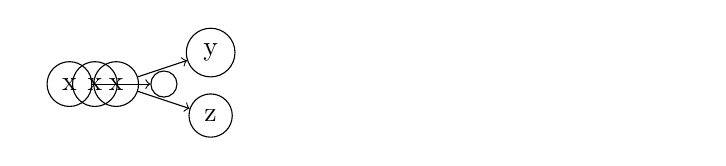
\begin{tikzpicture}
                \graphbox{$L$}{0mm}{0mm}{30mm}{20mm}{0}{0}{
                    \node[draw,circle]  (x) at (-6mm,-12mm) {x};
                    \node[draw,circle] (y) at (6mm,-12mm) {};
                    % \node[draw,circle]  (z) at (6mm,0mm) {};
                    \draw[->]  (x) to (y);
                    % \draw[->] (y) to[bend right=20] (z);
                    % \draw[->]  (z) to[bend right=20] (y);
                }
                \graphbox{$K$}{40mm}{0mm}{30mm}{20mm}{0}{0}{
                    \node[draw,circle]  (x) at (-6mm,-12mm) {x};
                    % \node[draw,circle]  (y) at (6mm,-12mm) {y};
                }
                \graphbox{$R$}{80mm}{0mm}{30mm}{20mm}{0}{0}{
                    \node[draw,circle]  (x) at (-6mm,-12mm) {x};
                        \node[draw,circle]  (y) at (6mm,-8mm) {y};
                        \node[draw,circle]  (z) at (6mm,-16mm) {z};
                        \draw[->]  (x) to (y);
                        \draw[->]  (x) to (z);
                }
                \node () at (35mm,-12mm) {$\leftarrowtail$};
                \node () at (75mm,-12mm) {$\rightarrowtail$};
            \end{tikzpicture}
        }
    \end{center}
    The set \( D(R,X) \) contains exactly two elements $R'$:
    \raisebox{2pt}{ 
        \scalebox{0.6}{\tikz[baseline=-0.5ex]{
        \node [draw,circle] (x) at (0,0) {x};
        \node[draw,circle] (y) at (1,0) {y};
        \draw[->] (x) -- (y) {};
    }}} and $R''$:\raisebox{2pt}{ 
        \scalebox{0.6}{\tikz[baseline=-0.5ex]{
        \node [draw,circle] (x) at (0,0) {x};
        \node[draw,circle] (y) at (1,0) {z};
        \draw[->] (x) -- (y) {};
    }}}. 
    Despite unique monomorphisms \( h_{R'L}: R' \rightarrowtail L \) and \( h_{R''L}: R'' \rightarrowtail L \) preserving interface elements, they fail the third condition of~\autoref{subgraph_counting:def:creates_more_x_on_the_left}. 
    For any rewriting step using this rule, implicitly created $X$-occurrences with the same subgraph of the context have the same corresponding $X$-occurrence. 
\end{example}
 
\begin{example}
    \label{subgraph_counting:ex:cond4_necessaire} 
    Let $X$ be the graph 
    \tikz[baseline=-0.5ex]{ 
            \node (x) at (0,0) {$\bullet$}; 
            \node (y) at (1,0) {$\bullet$};
            \node (z) at (2,0) {$\bullet$};
            \draw[->] (x) -- (y)   {};
    }, which has an isolated node. The following rewriting rule is potentially $X$-increasing.
    \begin{center}
        \resizebox{0.6\textwidth}{!}{
            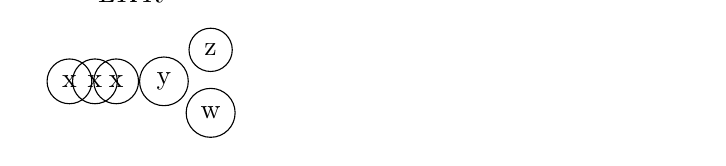
\begin{tikzpicture}
                \graphbox{$L$}{0mm}{0mm}{30mm}{20mm}{0}{0}{
                    \node[draw,circle]  (x) at (-6mm,-10mm) {x};
                    \node[draw,circle] (y) at (6mm,-10mm) {y};
                }
                \graphbox{$K$}{40mm}{0mm}{30mm}{20mm}{0}{0}{
                    \node[draw,circle]  (x) at (-6mm,-10mm) {x};
                }
                \graphbox{$R$}{80mm}{0mm}{30mm}{20mm}{0}{0}{
                    \node[draw,circle]  (x) at (-6mm,-10mm) {x};
                        \node[draw,circle]  (y) at (6mm,-6mm) {z};
                        \node[draw,circle]  (z) at (6mm,-14mm) {w};
                }
                \node () at (35mm,-10mm) {$\leftarrowtail$};
                \node () at (75mm,-10mm) {$\rightarrowtail$};
            \end{tikzpicture}
        }
    \end{center}
    The set \( D(R,X) \) contains exactly two elements $R'$:
    \raisebox{2pt}{\scalebox{0.6}{\tikz[baseline=-0.5ex]{
        \node [draw,circle] (x) at (0,0) {x};
        \node[draw,circle] (y) at (1,0) {z};
        % \draw[->] (x) -- (y) {};
    }}} and $R''$:\raisebox{2pt}{\scalebox{0.6}{\tikz[baseline=-0.5ex]{
        \node [draw,circle] (x) at (0,0) {x};
        \node[draw,circle] (y) at (1,0) {w};
        % \draw[->] (x) -- (y) {};
    }}}. 
    There are unique monomorphisms $h_{R'L}:R' \rightarrowtail L$ and $h_{R''L}:R'' \rightarrowtail L$ preserving interface elements, but they fail the fourth condition of~\autoref{subgraph_counting:def:creates_more_x_on_the_left}.
    For any rewriting step using this rule, implicitly created $X$-occurrences with the same subgraph of the context have the same corresponding $X$-occurrence.
\end{example}


\section{Solution to the key challenge}
\label{subgraph_counting:sec:solution_to_the_key_challenge}
The following lemma (see \iflongversion
% \hyperref[proof:lem:w_u_l_not_geq_r_not]{Section C}
\textsection~\ref{proof:lem:w_u_l_not_geq_r_not}
\else
\cite[Lemma 40]{qiu2025termination}
\fi for a proof) ensures that if $\rho$ is $X$-non-increasing, then, for any rewriting step using $\rho$, 
more X-occurrences are implicitly destroyed than implicitly created by the rewriting step.
% the cardinality of the set of \( X \)-occurrences implicitly destroyed by the rewriting step is at least as large as the cardinality of the set of \( X \)-occurrences implicitly created by the rewriting step.
% There are more implicitly destroyed X-occurrences than implicitly created X-occurrences.

\begin{lemma} 
    \label{subgraph_counting:lem:w_u_l_not_geq_r_not}
    \ \newline 
    \noindent 
    \begin{minipage}{0.7\textwidth}
        Let $X$ be a ruler-graph and $\rho = (L \overset{l}{\leftarrowtail} K \overset{r}{\rightarrowtail} R)$ an injective DPO rewriting rule.
        Suppose that $\rho$ is $X$-non-increasing. For every rewriting step induced by the DPO diagram (shown on the right), we have 
        \[
            |\operatorname{Mono}(X, G, \lnot m, \lnot l')| \geq |\operatorname{Mono}(X, H, \lnot m', \lnot r')|
        \]
    \end{minipage}
    \hfill
    \begin{minipage}{0.29\textwidth}
        \hfill
        \resizebox{0.9\textwidth}{!}{
                \begin{tikzpicture}
            \node (k) at (0,1) {K};
            \node (l) at (-2,1) {L};
            \node (r) at (2,1) {R};
            \node (c) at (0,-1) {C};
            \node (g) at (-2,-1) {G};
            \node (h) at (2,-1) {H};
            \draw[<-<]  (l) -- (k) node [midway,below] {l};
            \draw[>->]  (k) -- (r) node [midway,below] {r};
            \draw[>->] (c) -- (g) node [midway, above] {l'};
            \draw[>->] (c) -- (h) node [midway,above] {r'};
            \draw[>->] (l) -- (g) node[midway, right] {m};
            \draw[>->] (r) -- (h) node[midway, left] {m'};
            \draw[>->] (k) -- (c) node[midway, left] {};
            \node () [at=($(l)!0.5!(c)$)] {PO};
            \node () [at=($(r)!0.5!(c)$)] {PO};
        \end{tikzpicture}
        }
    \end{minipage}
\end{lemma}
